\chapter{Scenarios of change} 
\label{Chapter8}
% 
% {\color{red} Message to supervisors: please take a look at the structure and
% ideas in this and highlight the good the bad and the ugly --- where should I
% focus my efforts most to wrap-up this chapter?}

% \lhead{Chapter 8. \emph{Scenarios of change}} % Write in your own chapter
\fancyhead[RO,LE]{Chapter 8. Scenarios of change} %2side
\fancyhead[RE,LO]{\thepage}

\begin{quote}
\textit{ ``In the 1970s, I used to wait for a break in the lines
of car-plant workers cycling to work on their bikes so that I
could cross the road to get to school. Today, there are almost
no workers employed by that factory any more; much of the work is done by
robots ... So much has changed so quickly''}
\end{quote}
\begin{flushright}
\citet[p.~106]{dorling2013population}
\end{flushright}

\begin{quote}
\textit{``There is no certainty where one can neither apply any of the
mathematical sciences nor any of those that are based on the mathematical
sciences''}
\end{quote}
\begin{flushright}
Leonardo da Vinci, \emph{Manuscript G}, quoted in
\citep[p.~13]{rosci1978hidden}
\end{flushright}
% Things I'd like to do in this chapter:
% - The likely energy savings of simple things:
% -- Dutch rates of cycling to work!
% -- Telecommuting amongst certain sectors of the population
% -- Modal shift vs distance

The preceding sections focus on
understanding the energy costs of commuting currently (based primarily on the
2001 Census, which may be considered out of date). The analysis so far has a
number of important policy implications in the present, %!!! footnote!
but transport systems are constantly evolving. It is the evaluation of
change
% , for example in infrastructure, policies and prices, on transport patterns,
that make transport models so useful to policy-makers. This chapter
therefore 
investigates the impacts of change on commuting systems.
More specifically, the focus is on evaluating the effects of changed
\emph{behaviour} on commuter energy use.
Behaviour was chosen in preference to other types of change,
such improved efficiency of vehicles due to new technology or new
infrastructure (which in itself can be an agent of change), for two main
reasons. The first is policy-related:
behavioural change is at the top of the `sustainable transport
hierarchy' (in the form of demand reduction and modal shift) proposed by
the Sustainable Development Commission (\cref{fsdc}, \cref{Chapter2}).
Changed behaviour can be brought about quickly at low cost, whereas
technological and infrastructural interventions tend to take longer.
Despite these advantages, which are reinforced in a time of fiscal constraint,
the energy impacts of behavioural shifts have received little attention,
relative to the energy impacts of new technologies such as electric cars.
% Second, this thesis does not seek to model and understand the impacts of
% specific interventions on commuting behaviour (this important area
% has received much attention already,
% as outlined in \cref{s:commuting}), but to provide a framework for evaluating
% the impacts of changes that are anticipated results of policy intervention on energy use.
Second, the impact of new policies on behaviour is itself subject to a high
degree of uncertainty: taking behaviour change as a given and building
on this (without worrying about how that change is brought about)
thus simplifies the modelling process and reduces the number of assumptions
on which it is based. 

In developing the scenarios of change, the
aim is not to create the most likely scenarios possible, or even the
optimal ones, but the most \emph{informative} ones. The task is twofold:
to inform about the likely energy impacts of specific types of behaviour change
(modal shift, telecommuting and localisation of economic activity) and,
secondly, to inform about \emph{how} spatial microdata can be harnessed,
in general terms, for policy evaluation in relation to commuting. The scenarios
are presented as idealised cases of what \emph{could} happen, not what
\emph{will} or \emph{should} happen. Consideration of how these changes are
brought about and which interventions most likely happen are omitted: it is
assumed that these details can best be provided by policy makers well-acquainted
with their plans or by researchers modelling the various factors that determine
commuting behaviour (\cref{s:commuting}). % Reluctance to make assumptions a prob?
% using the
% method to evaluate concrete proposals.

A basic concept in modelling, embodied in the principle of parsimony
often referred to as `Occam's razor',
is to use the simplest explanation wherever possible. This implies
modellers should start simply, only adding further complexity when
necessary \citep{batty1976urban}. \index{Occam's razor} It is vital when
using mathematical models to investigate complex systems to remember the
following point, that recurs in the literature \citep{Wilson1970, Smil1993,
MacKay2009}: the purpose of the exercise is not to capture the totality
of the system (this is impossible in a truly complex system), but to enhance
\emph{understanding} of the processes being modelled.
% !!! quote from Wilson1970
The real world is heterogeneous, so ``one size fits all'' models, with no
critical interpretation, are of little use. Models that are ``black
boxes'', and not set up for the particular (and often unique) problem that they
are designed to solve may even hinder understanding,
by letting the computer provide an answer with no insight into how or why it
arrived at the answer. ``In some senses, every
application of a model is unique and requires special adaptation to the
problem in hand, and thus there is an element of hypothesis testing in
every predictive model design'' \citep[p.~4]{batty1976urban}. It is when the
focus shifts away from testing, experimentation and understanding and towards
``generating the `right' result'' that models can become dangerous and
politicised.

For this reason, this chapter is structured so that the simplest 
scenarios are presented first, to ensure maximum transparency and
understanding.
% These are then followed by more complex model experiments.
There are
five subsections.
% an ex-ante case study of a travel %old...
% to work scheme in a large employer, modelling local transport infrastructure
% interventions (improved bus and bicycle infrastructure for travelling between
% Stocksbridge and Sheffield), quantifying oil vulnerability of commuter patterns
% under the scenario of oil price shocks, and a more complex scenario of
% localisation in economic activity.
The first two are named after the nations which inspired the 
scenarios contained within: `going Dutch' for modal shift to cycling;
`going Finnish' for uptake of telecommuting.
`Going Dutch' is implemented both at aggregate and individual levels,
to highlight the advantages of each approach: the aggregate level
scenario allows energy savings to be calculated nationwide, while the
individual level implementation allows more sophisticated determination
of the chances of switching mode based on continuous age and distance
variables, rather than the simple dependence on distance bands
assumed in the aggregate level version. The code used to generate and analyse
these scenarios is provided, for reproducibility and transparency, in the
`scenarios' folder of the `thesis-reproducible' repository published alongside
the thesis.\footnote{This is
available
{\color{blue}\href{https://github.com/Robinlovelace/thesis-reproducible}{online}
} from github and can be found by searching for
`thesis-reproducible' on the github.com website.}
\Cref{fecoloc} is concerned
with a more complex scenario which raises the issue of the limits to the
spatial microsimulation approach and modelling more generally. \Cref{svul}
explores another use of the model: for evaluating the
extent to which commuters are vulnerable to oil price shocks. Finally, in
\cref{fc8discus}, the policy relevant findings from the chapter are summarised
and the limitations of the approach as a decision making
tool are discussed in the context of future uncertainty.

\section{Modal shift: `going Dutch'} \index{mode of travel}
\label{smshift} % Call this scenario going Dutch!!!
\begin{quote}
\textit{''I've got three ways of getting to work. The bus, the car and the bike.
If I go
by car I know that if I leave between about 7:15 and 9 O’clock I'll get stuck in
a jam and there's no way round it. And then I've got to find somewhere to park.
If I go by bus, well the bus runs every 30 minutes and it gets stuck in the same
jams, except for the bit with the bus lane. But if I go by bike it takes about
the same time as the car for seven miles, I get exercise, I don’t have to wait
anywhere and, I know I shouldn't, but
I get this smug feeling when I overtake all the cars in the traffic jams. You
talk about the car as a symbol of freedom and independence - for me that’s my
bike, not the car!''}\end{quote}
\begin{flushright}
  (Anonymous commuter, \citealp[p.~61]{Goodwin1991a}).
\end{flushright} \index{bicycle}

The quote above demonstrates that the individual benefits of modal shift
to bicycles can be large, even before any of the direct and indirect energy
savings are considered. Perhaps because of these highly tangible benefits,
modal shift is seen by many as one of the main
ways to tackle energy intensive commuting. The recent announcement of
\pounds148 million (77 for 8 cycling cities, 71 distributed by local
authorities) in cycling expenditure by David Cameron underlines the perceived
benefits increased cycling.

Returning briefly to the basic comparison between the Netherlands and England
presented in \cref{tcompare}, it is clear that the two countries are relatively
similar, at least on paper. Using the former's famously high cycling rate of
25\% for all commutes, it would be possible to set this as a long-term goal for
UK cities. \Cref{sinternational} shows that a high rate of cycling does not
lead, on its own, to low overall commuter energy costs. Yet it does provide an
empirical basis for a what-if scenario of modal shift to cycling in England.

\subsection{An aggregate level model of modal shift}
Starting at the national level, let us make assumptions about the people who
transfer to cycling from other modes in a very high cycling uptake scenario,
for each Euclidean distance band. Because cars are the main culprit of energy
intensive commuting, and for the sake of simplicity, only the car-bike shift is
considered, after \citet{Lovelace2011-assessing}:\footnote{In
reality, it is likely that cycling
would have an equally high tendency to replace the other common modes of
short-distance travel --- bus
\citet{dorling2013population} and walking trips. The former is due to the
financial savings to be made, the latter due to the increased speed of cycling
over walking. It could be argued that neither of these shifts would have
substantial energy implications compared to the car-bike shift, however: bus
use and walking both constitute a lower share of commuting, even for short
trips than car trips; both are less energy intensive than driving (in the case
of walking, greatly so); and even if bus trips \emph{were} replaced by bicycle
trips for shorter trips, the energy savings that result would be highly
uncertain ue to the top-down nature of bus service planning --- it is largely
elderly citizens who are least able to cycle who most depend on bus services.
}
\begin{itemize} \index{bicycle}
 \item a 50\% shift for car journeys between 0 and 2 km
 \item 30\% shift for trips between 2 and 5 km
 \item 5\% of car commuters in the 5 to 10 km band shift, and
 \item just 1\% of car commuters in the 10 to 20 km band
 shift\footnote{This
 number is so low because, knowing long-distance (7 miles plus, each way),
 bicycle commuters, the trip is usually only taken by bike a few times per week
at most. In addition, this is far beyond the capabilities of the majority of
the population, so is still a very optimistic assumption.
}
\end{itemize}
These numbers are based on a loose interpretation of Dutch data: 43.6\% of
all trips between
1 and 2.5 km, and 33.3\% of trips up to 7.5 km were made by bicycle in the
Netherlands in the year 2000 \citep{Rietveld2004}.
Still, in the British context it is acknowledged that these values are quite
arbitrary and ambitious: peoples' uptake of cycling may be different in England.
50\% value for the shortest trips is certainly possible physically in most
areas, but would
take a transformation in travel to work habits for the 8\% of commuters who
travel 2 km or less by car (20\% of commuters travel this distance to work
overall). Evidence from the Netherlands and Denmark show that it
is possible for more than 30\% of \emph{all trips} (not just those less than 2
km) can be made by bicycle in some cities (Groningen, Munster, Copenhagen,
for example), provided the correct policies are in place \citep{Rietveld2004,
Pucher2010}.
In addition, an EU report concluded that 30-50\% of car trips below
5 km could be replaced by walking and cycling
combined.\footnote{``There
is a considerable potential of car trips of less than 5 km that could be
done by walking and cycling. The analysis carried out allows us to establish
that it lies between 30\% and 50\% in European countries''
\citep[p.~60]{Gnavi1999walcying}.
}
Beyond 5 km the drop-off is expected to be steep: cycling 6 miles of route
distance (roughly in the centre of the 5-10 km Euclidean distance bin) each way
each day requires a level of fitness and commitment held only by a few.
Cycle-commuting further than 10 km each day requires exceptional levels of
fitness, but is not unheard of, even in the current low-cycling
context.\footnote{The following comments
were taken from the online forum http://singletrackworld.com in response to
the question ``how far is too far to commute by bicycle each day?'': ``I found
that doing 20 miles a day (10 each way) for 5-6 days meant I was knackered for
any weekend riding.'' ``I do 23 miles each way but only twice a week. I don't
think I could do 5 days a week!''  ``when I was very fit, I found 19 miles each
way 5days a week fairly hard going though I've never been any good at just
cruising along.'' ``I've done 13 miles each way every day through London (so
lots of start stop) and that was ok most of the time. Done a asymmetric 17.5
miles there 13 miles back and that started to feel bit of a drag in terms of
time and and effort. I think for me 15 miles each way would be my limit for 5
days a week.
Although at the moment I'm very lazy and drive 8 miles to work 3 days a week and
ride ride 2days a week!''
}
Based on these assumptions it is possible to calculate the energy savings from
a modal shift to cycling:
\begin{equation}
 \Delta Etrp = \sum_{b} p_b \times \overline{EI}_{car,b}
\overline{dR}_{car,b} \times N_{car,b} - p_b \times \overline{EI}_{bike,b}
\times \overline{dR}_{bike,b} \times N_{car,b}
\end{equation}
where $b$ are distance bands (in this case from 0-2 to 10 to 20 km), $p$ is
the proportion of car trips replaced by bicycle trips, $EI$ is the energy
intensity of travel (MJ/km, from \cref{Chapter5}), $dR$ is the route distance
and $N$ is the number of people travelling by that particular mode-distance
combination. \index{bicycle}

Applied across England (simplifying to assume $EI$ remains constant over all
distance bands considered), this analysis suggests that the average energy
costs of commuter trips could be reduced by 3.2\% nationwide. Clearly, these
are optimistic assumptions about uptake of cycling, so the true figure
offered by modal-shift to bicycles in the short-term is likely to be
lower. However, because the majority (60\%) of commuters travel
over 5 km, beyond which only a handful of drivers will switch to bikes, the
proportion of all trips is not as high in this scenario as might
have been expected: it increases from 2.1\% currently to 10.1\% in the high
cycling scenario --- still far less than the 25\% figure for Dutch cycle
commuters, and well below the rate of cycle commuting in the most cycle-friendly
areas of the UK. In the ward of Romsey, just east of central Cambridge, for
example, over 30\% of commuters cycle to work. 

Geographically, the energy savings of this what-if scenario vary considerably.
At the regional level, savings would be highest in the Northwest and lowest in
the East of England (3.7 and 2.5\% respectively).
At a lower levels, a clear geographical pattern emerges: the potential energy
savings of replacing car commutes with bicycles tend to be greatest in the
urban areas directly surrounding town and city centres. Beyond around 5 miles
from city centres, the potential energy savings drop rapidly to below the
national average. Potential energy savings in central wards tend to be slightly
lower than this ring of between around 1 and 5 km from the city centre.
This pattern is clearly present in \cref{fcysave}, which shows the results in
the region of Yorkshire and the Humber. From the perspective of transport
planning, this result could be extremely useful for allocating cycling
investments to areas where it would have most impact.
In general, the results seem to support the prioritisation of routes into
city centres from the outskirts. It would be an interesting exercise to assess
the extent to which current bicycle path geography reflects areas of highest
potential energy savings.

\begin{figure}
 \centering{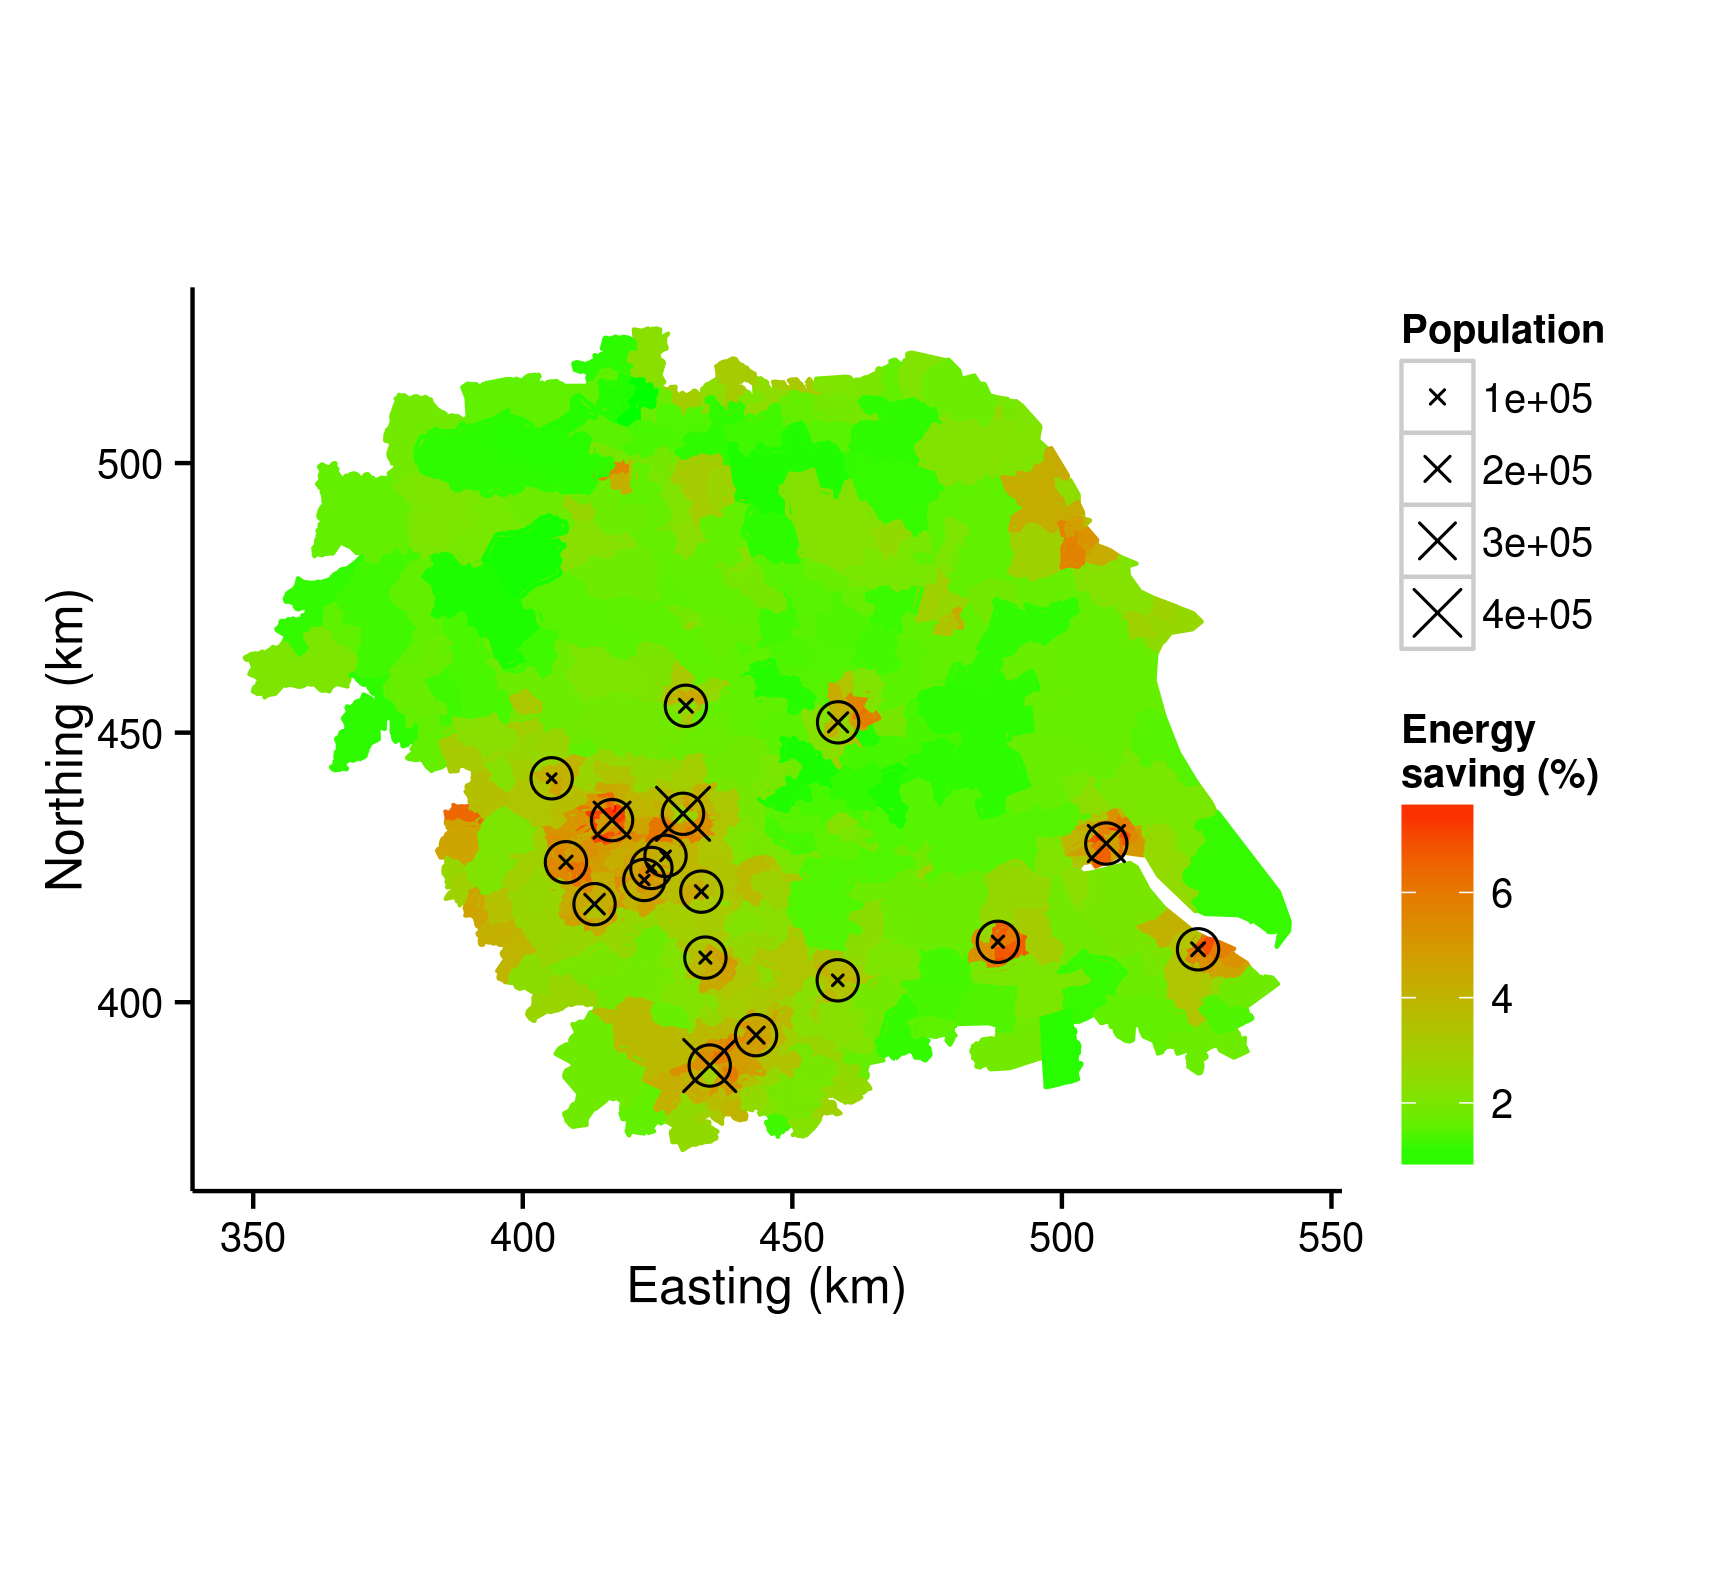
\includegraphics[width = 12cm]{cysave}}
 \caption[Estimated energy savings from car-bicycle modal shift]{Estimated
energy savings from car-bicycle modal shift in Yorkshire and the Humber at the
Ward level. Size of x points represent size of settlements with over 30,000 people,
rings illustrate circle 5 km from city centres.} \label{fcysave}
\end{figure}

The above results are based on crude assumptions and simple
back-of-the-envelope calculations. They take no account of the characteristics
of the people in each zone (young people, for example are more likely to be
willing to take up cycling), infrastructure or terrain. A number of refinements
could be made, based on simulated spatial microdata and information about the
environment in each zone. Based on the literature, socio-demographic,
infrastructural and environmental factors all play a role in determining the
cycling rate. Thus, using the spatial microsimulation approach, the shift to
cycling could be modelled at the individual level, as a function of
individual and geographical factors, for example:
route distances (for cars and bicycles), topography, climate, age, sex,
the price of driving and perceived attractiveness of cycling. 
% \begin{equation}
%  Pr = f(dR_{car}, dR_{bike} topo, climate, age, sex, bikepath, pricedrive,
% attractbike)
% \end{equation}
\subsection{A spatial microsimulation implementation}
% !!!
The simplistic assumption that a fixed proportion of car commuters will
shift to bicycle for each distance band in all areas is clearly flawed.
As mentioned above, a range of factors conspire to influence the number of
people cycling in any given area. The physical ability to ride a bike
has a strong age dependence and it is well-known that the current wave
of cycling uptake is driven largely by the
young.\footnote{Sex
may also impact the probability of bicycle uptake: ``Gender may be an issue when
women have to consider the social risks of travelling by bike during the
evening'' \citep[p.~532]{Rietveld2004}, but this reasoning is not deemed
strong enough to merit a gender dependence here.
}
Some areas will have a higher proportion of older commuters, who would
be less likely to be able, physically, to cycle a long distance to work.
An additional problem with the aggregate level model is that it depends
on distance/mode cross-tabulations, which are not available at all
geographic levels.

It is precisely this context, of multiple and interacting variables
affecting an output, operating on individual to regional levels,
that spatial microsimulation becomes useful. In this implementation,
the outputs of the spatial microsimulation technique set out
in \cref{Chapter4} are used to create an individual level model of modal shift.
To take the age-dependence into account, the individual level implementation
of the `Going Dutch' was undertaken as follows:
\begin{itemize}
\item The probability of switch to bicycle depends on \cref{fimpedance}
set out in \cref{eimpedance}.
The ``cycle to work'' parameters from
\citet{Iacono2010} were used: $\alpha = 0.402$; $\beta = 0.203$.
% The parameter x and y depend on age, leading to the following
% probability distribution.
\item The age dependence of the shift was estimated based on the National
Travel Survey data: the 
relationship between variable i272 (``Ridden a bicycle in the last 12 months'')
was determined as a linear function of age (see \cref{fpriden}) and this
simple linear model was used to normalize the previous probability
estimates by age.
\item The sample size was set equal to the modal shift resulting from the
aggregate level implementation of the `go Dutch' scenario, with the probability
of switch depending on age and distance, as described in the previous bullet points.
\item The energy savings of a switch were calculated and aggregated for each zone.
\end{itemize}

\begin{figure}
 \centering{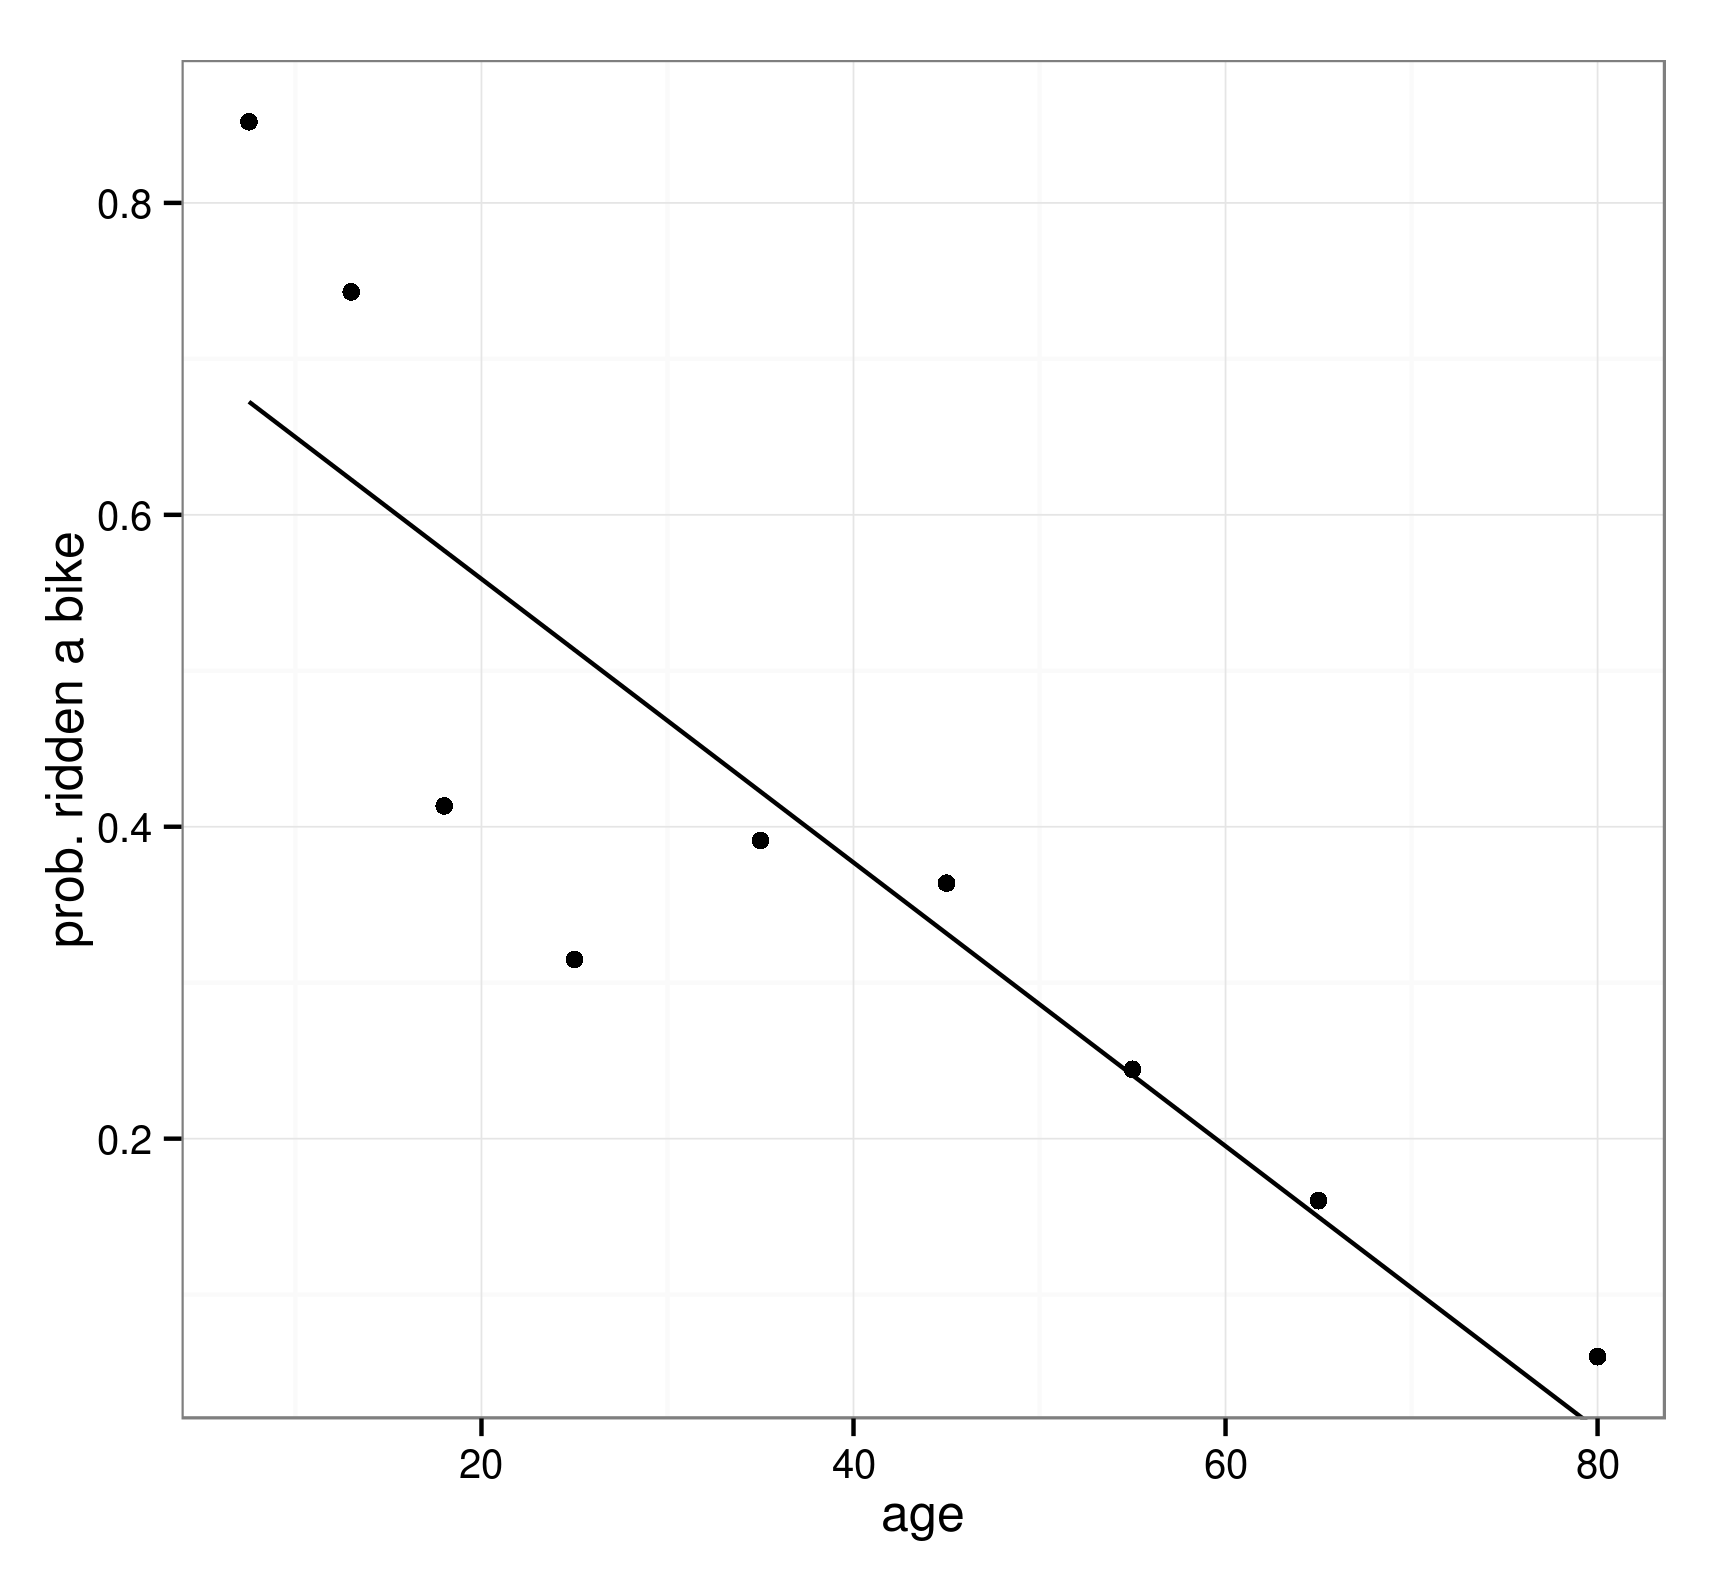
\includegraphics[width = 12cm]{priden}}
 \caption[The relationship between age and bicycle use]
 {The relationship between age and bicycle use, from the National Travel Survey.
 Ordinary Least Squares regression was used to find how the probability
 of having cycled in the past year (y axis) related with age --- it was assumed
 to be linear after visual inspection. The resulting formula was $p = 0.74 -
 0.0091 \times age$. 
 } \label{fpriden}
\end{figure}

Applied to South Yorkshire overall, the energy savings resulting from this
scenario were 4.0\% of total energy use, slightly above the national average.
As with the national level figures, the savings vary geographically: the lowest
energy savings were found in the city centres (most notably Sheffield's),
where cars are rarely used for short distance trips (walking and public
transport options are already popular). The areas of highest energy savings
tended to be found in annuli (rings) surrounding urban centres, with inner and
outer bounds approximately 2 and 5 km from the centres respectively (\cref{fbikeage}) .

\begin{figure}
 \centering{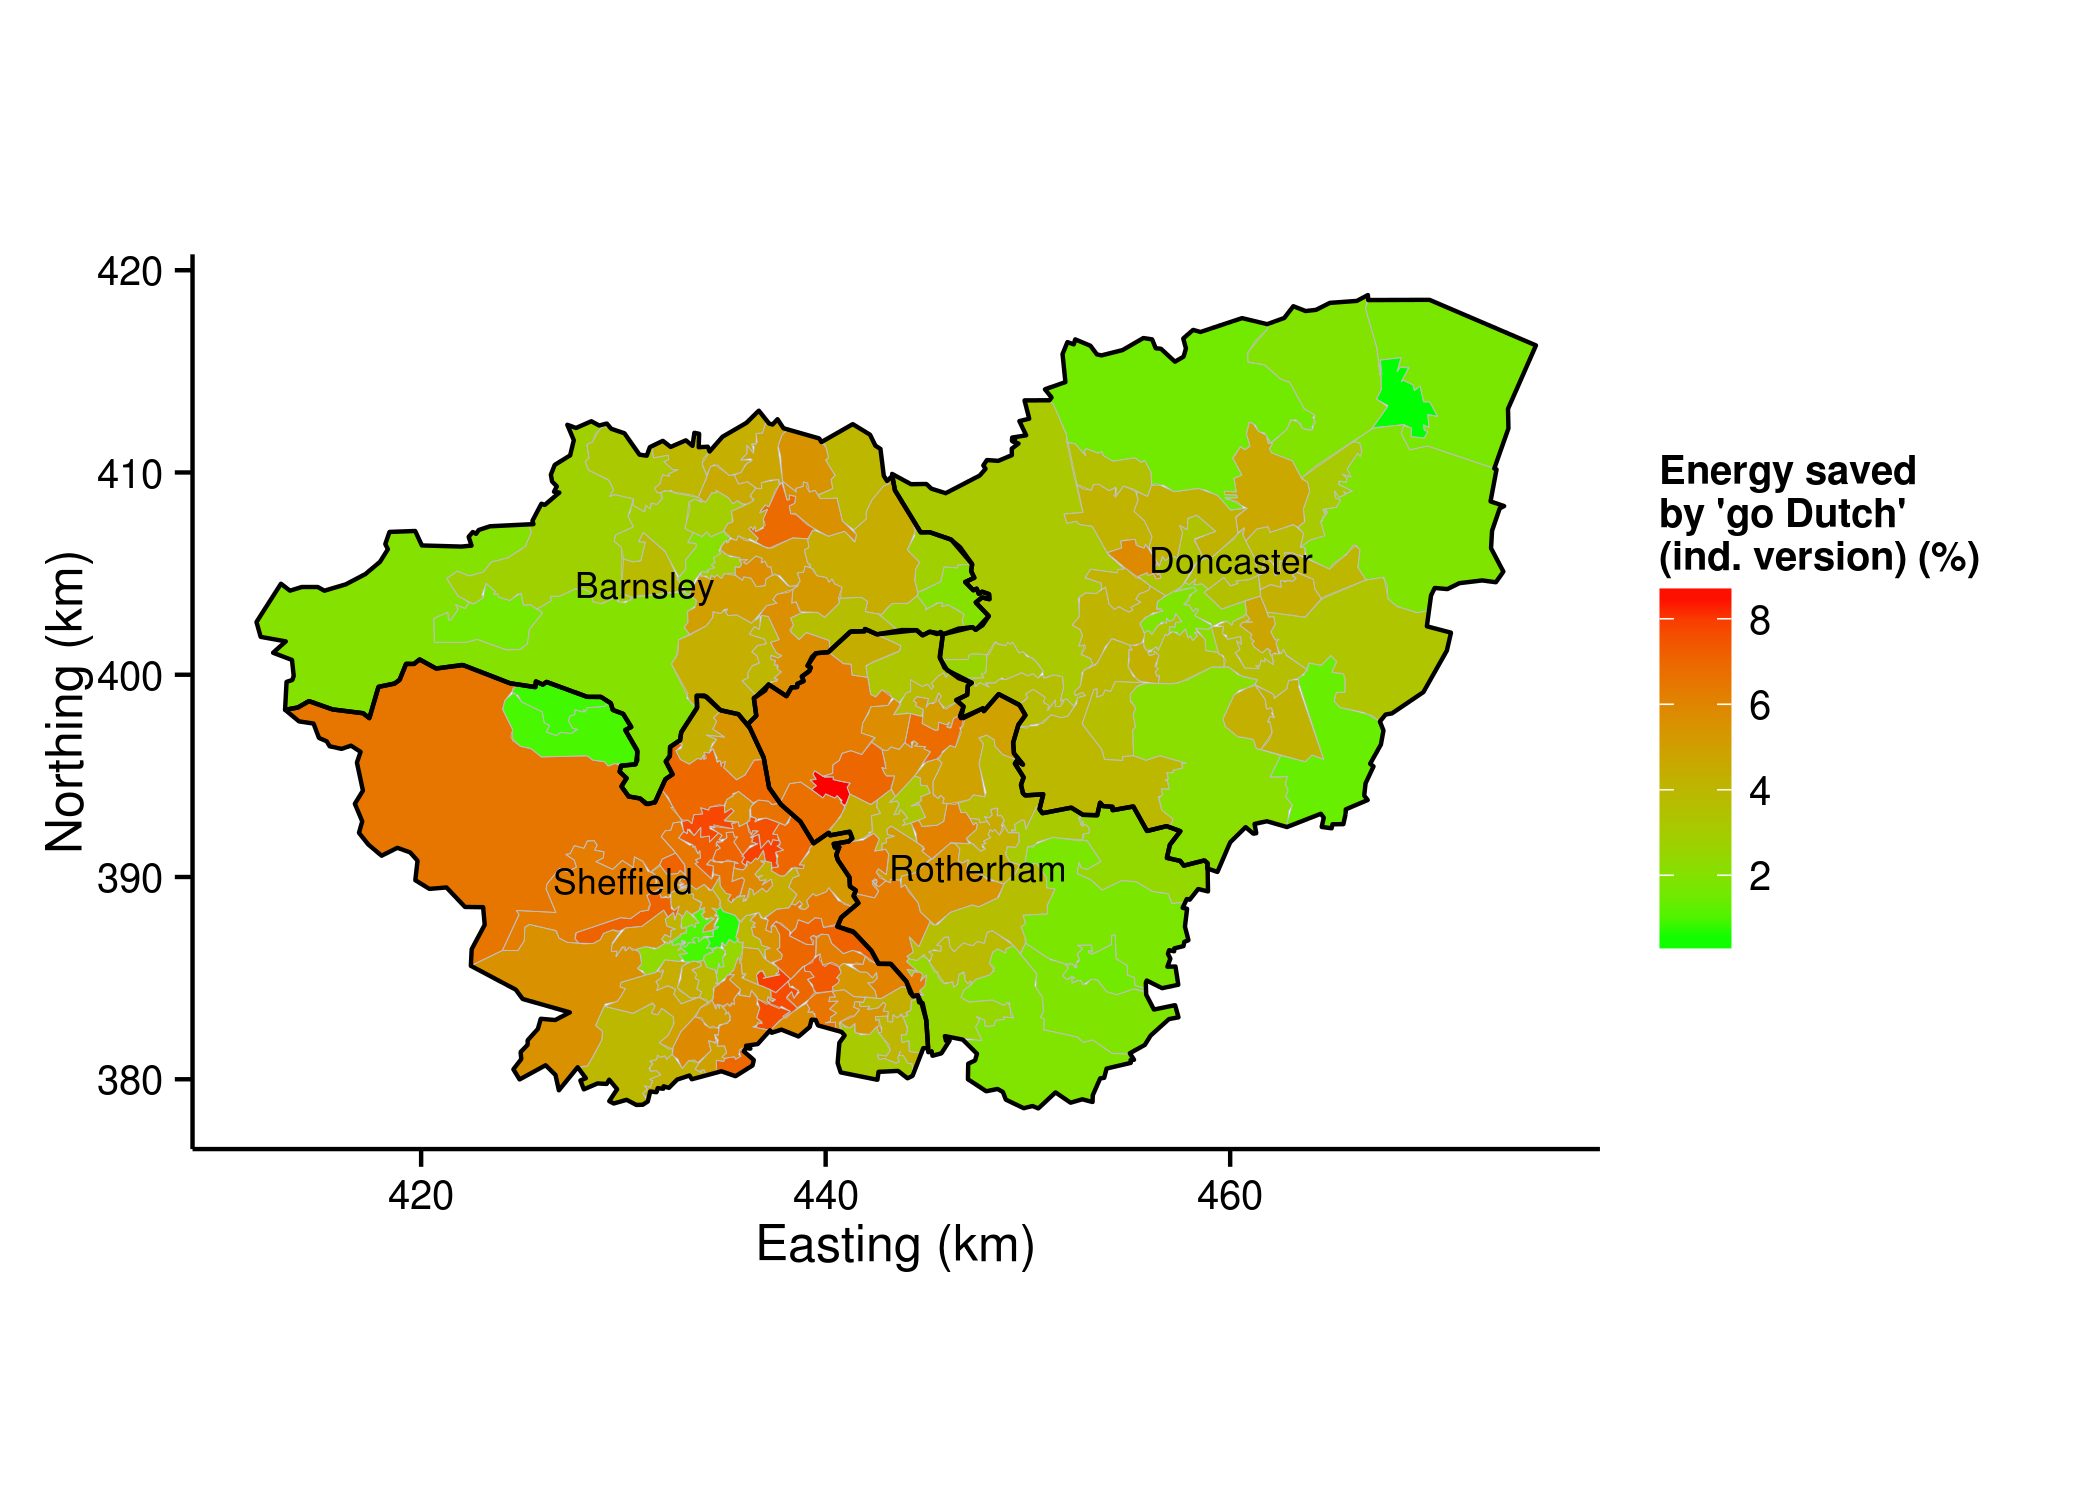
\includegraphics[width = 12cm]{cysave-ind}}
 \caption[Energy savings from car-bike modal shift in South Yorkshire]
 {Energy savings from car-bike modal shift in South Yorkshire, from the
 individual level implementation of the `go Dutch' scenario.} \label{fbikeage}
\end{figure}

Across the region as a whole, the difference between the individual level
implementation (with age dependency) and the simplistic implementation
(without age dependency and probability bands, not a continuous probability
variable dependent on distance) was small: energy savings were 4.4\% in the
simplistic model, 0.4\% percentage points greater. This can be explained by the
range of distances within distance bands: in the individual level implementation
a 9 km trip is less likely to switch to bicycle than a 6 km trip whereas
in the aggregate level model the probability is the same. The spatial distribution
of the differences between the estimated energy savings in the individual level
and aggregate level implementations are shown in \cref{fcydif}. Note that the
individual level savings were substantially lower in Stocksbridge (Northwest
Sheffield).

An interesting feature of the `go Dutch' scenario is that more energy is
saved in areas with below-average commuter energy costs than in areas where
commuter energy costs are high. (In the individual level implementation
displayed in \cref{fbikeage}, the correlation between current commuter energy use
and predicted savings was -0.20, a statistically significant result).
This can be explained in terms of distance:
areas with the highest energy costs will tend to be too far from
commuter centres for cycling.
% One hypothesis for this could be that, a zone
% historically dependent on the steel industry,
% many of the people who now commute into work are older, whereas young
% people who get jobs elsewhere tend to leave.

\begin{figure}
 \centering{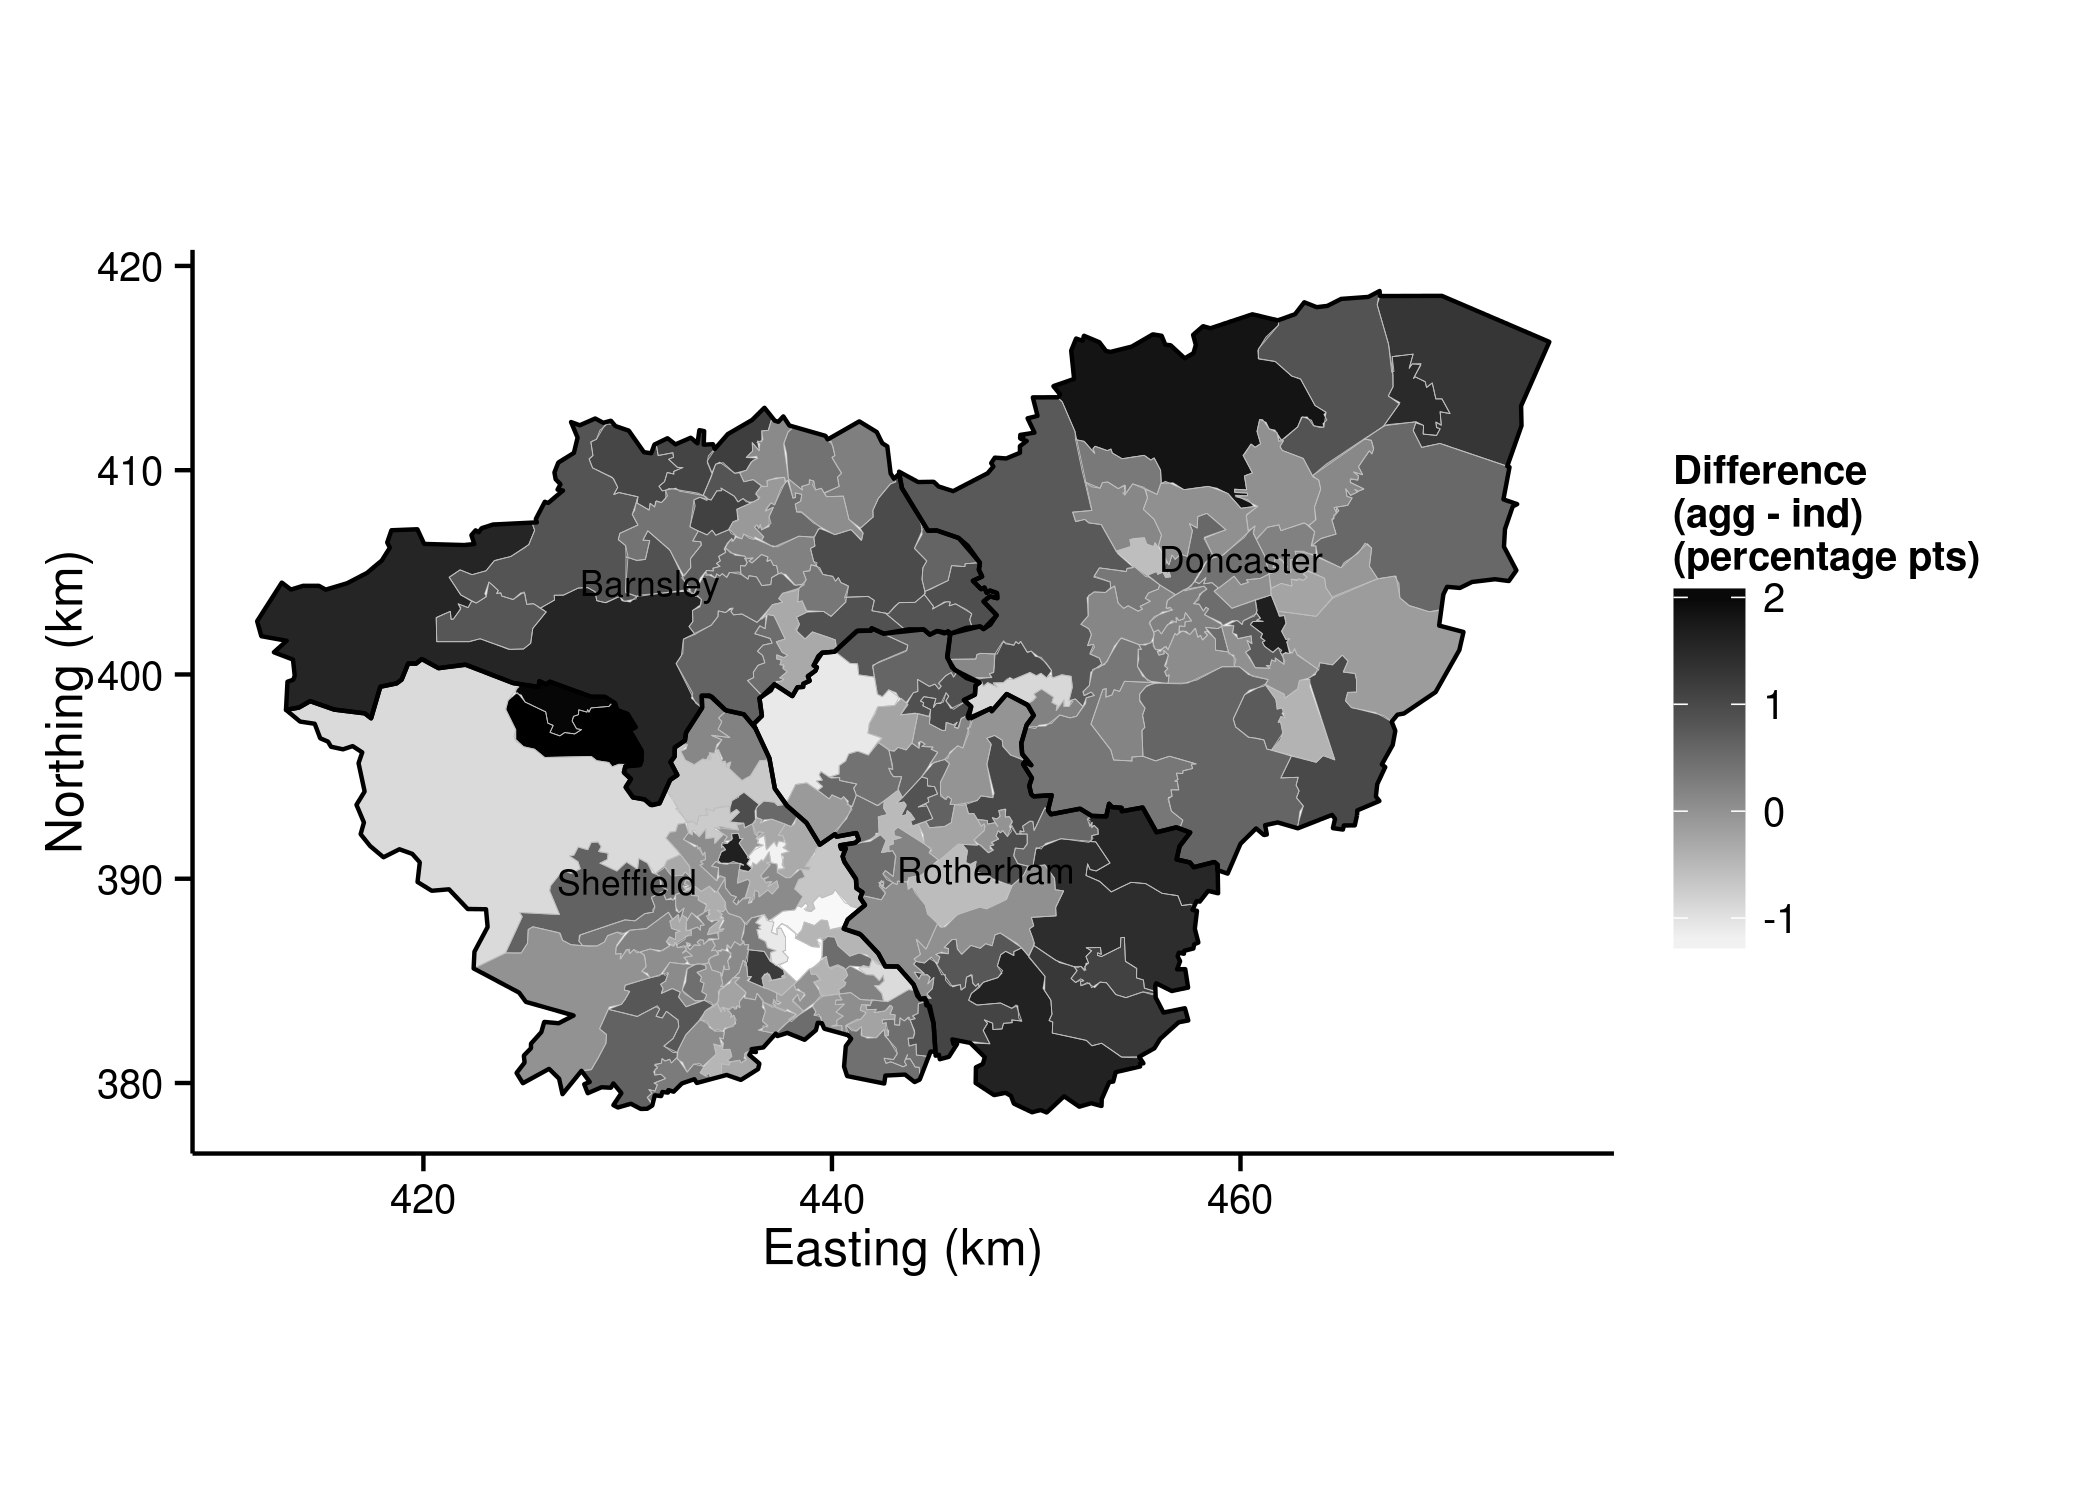
\includegraphics[width = 12cm]{cysave-diff}}
 \caption[Differences between individual and aggregate level implementations]
 {Differences between individual and aggregate level implementations of the
 `go Dutch' scenario across the MSOA zones of South Yorkshire.} \label{fcydif}
\end{figure}

\subsection{Taking the scenario further} \label{stfurther}
Using methods akin to the binomial regression model presented in %!!! basically discussion!
\citet{Schoner2013}, the probability of a car-driving commuter switching to bicycles
could be calculated. Proxies for the more ambiguous quantitative concepts such as
`topography'
(e.g. the proportion of land area with a slope greater than more than 3\% ---
see \citep{Heinen2012}), climate variables (e.g.~number of days of rain per
year), could be constructed. The model could be calibrated based
on existing data, and then used to evaluate specific what-if scenarios.
A new bicycle path, for example, could alter both $dR_{bike}$ and $bikepath$
variables; carbon taxes could increase the price of driving, whereas new cycle
facilities could increase the attractiveness of cycling, for any particular area.
\citet{Buehler2012} specified and ran such a logit model to investigate the
impact of cyclist facilities on cycling in Washington.
Such an approach, based on
spatial microdata, would signify a major step forward
in the sophistication of models of modal shift for policy evaluation from the
city-wide population model used by \citet{Lovelace2011-assessing} to estimate the energy
savings resulting from cycling uptake in Sheffield.

It is outside the scope of the thesis to design and
implement this model. However, the approach has great potential for
assessing individual schemes in terms of energy use and extending
non-geographical work on modal shift \citep{Lovelace2011-assessing}. The main barrier
to the implementation for practical transport planning purposes
would be not so much the accessibility of data from which it could be tested
and calibrated, but expertise and time to create suitable spatial microdata
with origin-destination points and accurate zonal and individual level
variables. Developing such a model would be an application of the spatial
microsimulation approach to assessing the energy costs of commuting with
important practical consequences. Indeed, a similar approach could also be used
to investigate the reduction of home-work distance, another oft-cited strategy
for reducing commuter energy use.

\section{Reducing commute frequency: `going Finnish'}
If modal shift to active modes has less impact than expected, perhaps
trip frequency is key. With the spread of high-speed internet over the
past two decades and the shift to service sectors over the past century,
the need to be physically present at work \emph{every day} for many people
has
diminished.\footnote{To
take one anecdotal line of evidence, my girlfriend Carlota works for Skype.
They are totally free to work wherever they want: there is no obligation to
be in the office each working day. The office is seen as a useful social hub
than the basis of productivity. In this case it would be hard to argue that
telecommuting reduces energy use (many of the staff spend time away from the
office on international trips), but it at least shows the potential of large
organisations to implement and even encourage long-distance work.
}
This section therefore focusses on telecommuting. The energy implications are clear:
Although the energy calculations made so far are on a per-trip basis, the
overall energy costs of commuting depend on how frequency the trip is made.
An individual who commutes 5 miles 200 times per year, for example, may
use more energy than someone who makes a 10 mile trip on a part-time basis.
These frequency estimates are not made in the model because the spatial
microdata is not constrained by hours of work (or even full-time/part-time
status). However, it is still possible to estimate the distribution of
energy savings resulting from telecommuting based on the obviously incorrect
but analytically useful assumption that everyone travels to work the same
number of times each year. This assumption can be made without a large impact
on the results because the major factor determining energy savings from
telecommuting will probably not be the prevalence of full/part time work, but
the possibility and willingness of people living in each zone to work from home.
This appears to be largely determined by distance to
work\footnote{\citet{Helminen2007}
found that the probability of telecommuting increased roughly exponentially
with increased distance, reaching a maximum of $p=0.12$ for individuals travelling
150 km to work
}
and type of job. In Finland, for example, ``teleworking was almost non-existent
among employees with a low educational level and manual work,'' whilst those
with higher occupational positions were far more likely to telework
\citep[p.~336]{Helminen2007}. Due to the lack of firm evidence about the
determinants of telecommuting in the UK, this information is taken as the
basis of the telecommuting scenario (which should certainly be updated
as more evidence emerges). Using the South Yorkshire simulated spatial microdata
described in \cref{Chapter7}, a simple interpretation of
\citet{Helminen2007} is used as the basis of energy savings. Thus, the scenario
was as follows:
\begin{itemize}
 \item Identify individuals in the highest socio-economic class, who are thought
 to be likely to be able to telecommute.
 \item Sub-sample from these, with the probability of selection set as
 $p = 1/e^{-y}$, where $y = −5.3 + 0.022 \times dR$ (measured in km) (see
 \citealp{Helminen2007}) and the sample size proportional to the number of
 higher occupation workers.
 \item Create a new energy cost estimate for each area by subtracting the
 energy costs of the sampled individuals from the total.
\end{itemize}
This resulted in a 9.2\% energy saving overall, with substantial variation between
zones \cref{ftelesave}. What is fascinating about this result is the numbers
involved: whilst approximately 8\% of commuters were affected by the
modal shift scenario developed in the previous sector (with energy savings
of only 3\%), the numbers are almost reversed in this scenario: altering the
behaviour of only 2.7\% of commuters could, in this case result in energy
savings approaching 10\%.

\begin{figure}
 \centering{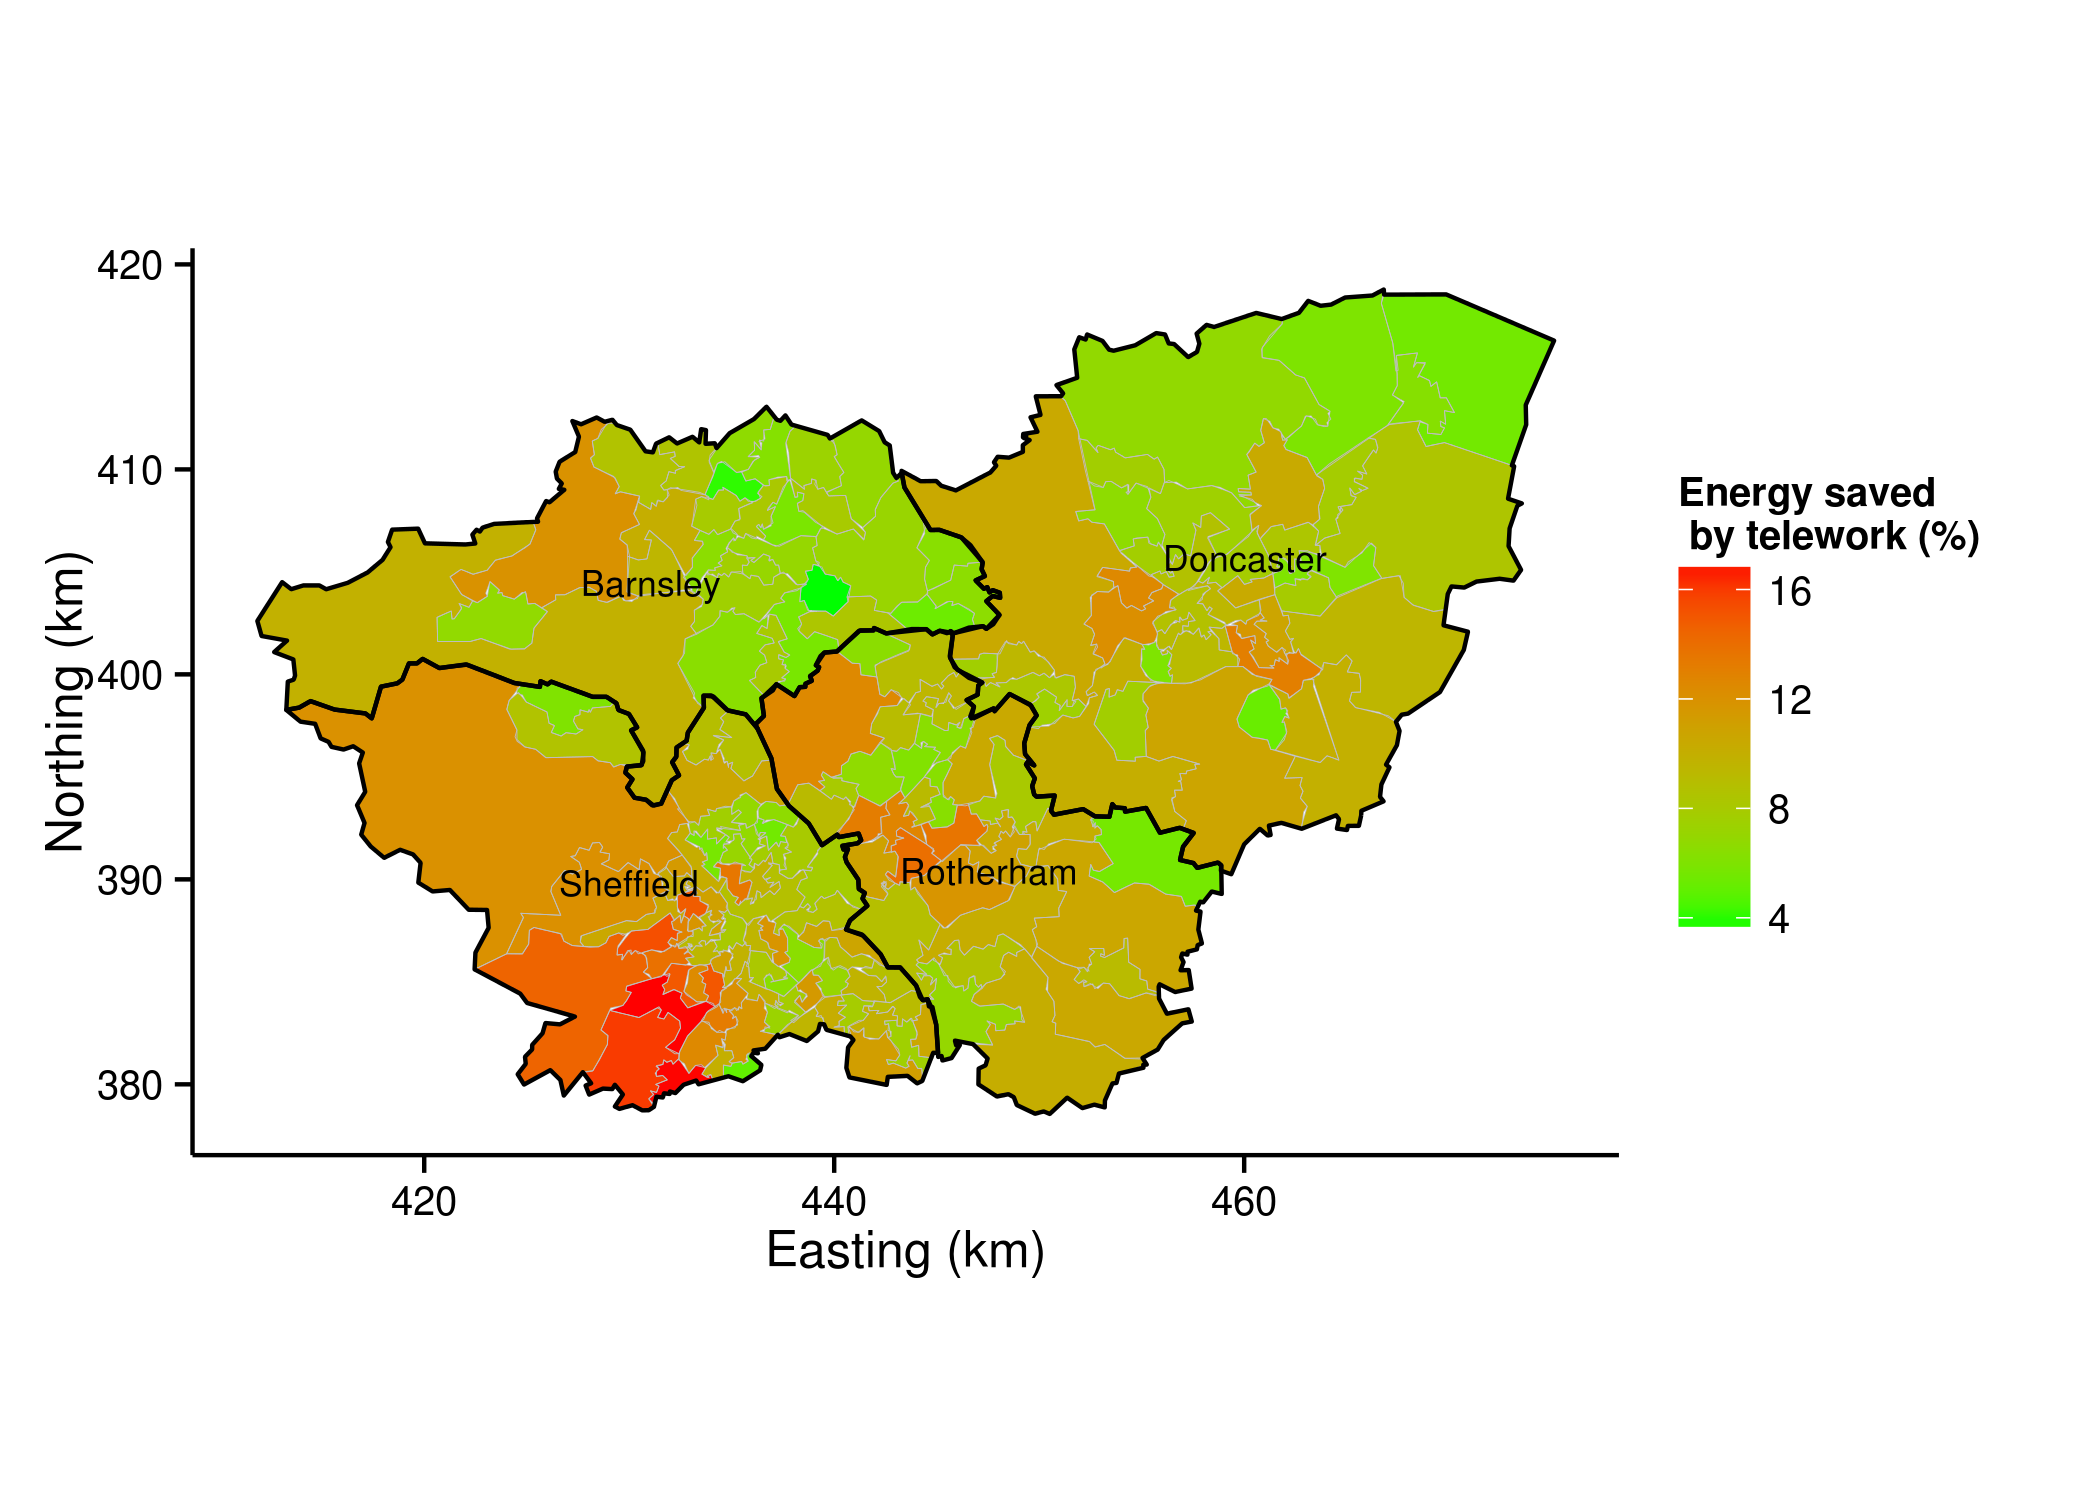
\includegraphics[width = 12cm]{telesave}}
 \caption{Energy savings from telecommuting scenario in South Yorkshire.}
 \label{ftelesave}
\end{figure}

The spatial distribution of energy savings reflects the areas of high wealth
(Dore in the West of Sheffield, for example is notoriously well off, and has large savings
in this scenario), long commuting distances and a preponderance of higher occupations
and managers. This is reflected in positive correlations between energy savings
and average trip length (r = 0.014, not significant), proportion of managers
and workers in higher occupations (r = 0.79, p $<$ 2.2e-16) and
mid-estimates of wealth for 2007-8 from the Office of National Statistics
(r = 0.63, p $<$ 2.2e-16). Unlike the modal shift scenario, the
greatest energy savings tend to be made in areas with high average energy
use for commuting, and affect the most energy intensive commuters rather than
the least.

Another current trend that has large potential energy implications is the
trend towards part-time work. Using similar methods as those presented above,
individuals likely to go part-time could be identified, and energy savings
could be calculated accordingly. Policies to promote this trend could
include reducing taxes for part-time workers. However, if the end result is the
same amount of work being done by more people, the energy savings
could be negligible, as more trips would be made by newly employed people.

\section{Reduction in commute distance: `eco-localisation'} \label{fecoloc}
% \subsection{Moving closer to work}
% \subsection{The localisation of economic activity}
The previous sections show that substantial energy savings can be made by
building on already existing social trends: towards pro bicycle and active
travel policies and telecommuting. However, savings of more than 12\% are needed:
the government has committed to reducing emissions by over 80\% by 2050
and given the slow pace of technological change \citep{Smil2010}, this
probably means large reductions in energy use. Of course, it would be possible
to develop more aggressive scenarios of modal shift and telecommuting for
South Yorkshire, but this section focusses on the `elephant in the room'
regarding energy intensive commuting: distance. As already suggested in
\cref{sinternational} and
emphasised by \citet{Boussauw2009}, home-work distance is the most important
driver of energy-intensive commutes. In the absence of nationwide high speed rail
or even an international
`hyperloop',\footnote{The
hyperloop was conceived by entrepreneur Elon Musk as a new mode of transport,
located somewhere between rail and aviation, faster than the former yet much
more energy efficient than the latter.
}
distance forces people to use the least efficient mode
(cars) and use them a lot. There is also a strong equality argument to
be made for focussing on distance: from the South Yorkshire case study,
only 7\% of commuters travel more than 30 km each day. Yet these individuals
account for 41\% of commuter energy use in the model. Failing very high
rates of telecommuting (with attendant social impacts),
this leads to the conclusion that home-work distances must be reduced to
cut dramatically energy usage for commuting.

How can this be done? Or more specifically for this research,
how can realistic scenarios of
reduced commuter distances be created? In the current economic context,
there are essentially only two options available to workers wanting a job
closer to home. These are: 1) move job or 2) move house. The former depends on
an adequate job being available closer to home, about which there is
an extensive literature, based around the concept of `excess commuting'
\citep{Buliung2002}.
The latter may not be feasible for financially constrained families,
due to the tendency of house prices to increase towards city centre, where
most jobs are to be found
\citep{Li2012},\footnote{Put in other terms,
commuters are ``trading off decreased house prices for longer commutes''
\citep[p.~312]{Li2012}.
}
but would be an option for the wealthiest commuters, who use a disproportionate
amount of total commuting energy use.

To realistically model this requires much information, including
the spatial variability
of house prices, its interaction with transport links and the availability
of specific types of job. This data could be obtained, to varying degrees,
and represented as part part of an integrated land-use transport model.
Spatial microdata could fit into this approach.
Yet the complexity of data and modelling is beyond the scope of this project.

Instead, the focus of this section is shifted to more hypothetical `what if' scenario
founded on the idea of the localisation of economic activity \citep{North2010585}.
% Based on this paper, this scenario is called `eco-localisation'.
The
premise of `intentional eco-localisation' is that ``responses to peak oil and resource
constraint as a long term problem cannot be disconnected from the
need to avoid catastrophic climate change'' \citep[p.~585]{North2010585} and its main
features are as follows:
\begin{itemize}
 \item Its proponents are not willing to wait for either new technologies or
 high oil prices to reduce energy use: lifestyles must change as part of an
 overall transition away from economic growth.
 \item Any economic activity that can be undertaken locally (e.g.~food production)
 will become increasingly
 decentralised (meaning that jobs less concentrated in specific areas).
 \item Suburbia in its current form gradually vanishes, and communities
 will become ```villagised' so people could meet more of their needs from their
neighbourhood without commuting'' \citep[p.~591]{North2010585}.
 \item Second locally useful professions will become common,
 to supplement conventional jobs further from home.
\end{itemize}
Of course, translating such a broad vision into a quantitative scenario
of change is highly challenging \citep{Winther2013}. This scenario
exists not only far in the future, but also under the assumption that
economic and social conditions will be very different from what they are today.
The socio-economic traits of individuals in South Yorkshire will also have
changed, reducing the relevance of the spatial microsimulation approach to this
problem.

% Nevertheless, a quantitative scenario was created. Unlike the previous two
% scenarios, `eco-localisation' is not designed to be feasible, but as a
% mechanism to explore ways of dramatically reducing the energy use of personal travel.
% The features of `eco-localisation' summarised above were translated into
% quantifiable changes to commuting in the follow ways:
% \begin{itemize}
%  \item 
% \end{itemize}
Based on these difficulties, and heeding the warnings from Vaclav Smil about the dangers
of creating arbitrary quantitative scenarios about the future of complex non-linear systems
\citep{smil2000perils, Smil2008}, it was decided to not quantify this scenario.
The costs of attempting to quantify energy savings of `eco-localistaion'
(the impression of simplicity and certainty, when in reality the long-term future
contains a vast array of possibilities) were deemed greater
than the benefits (potential clarification of the mechanisms by which it is assumed that
commuter energy costs would be reduced). The main benefit of quantitative
scenarios are for policy evaluation: unlike modal shift or telecommuting,
the `eco-localisation' scenario cannot be reduced to a single policy or change.

All this is not to say that one cannot imagine what the commuting pattern would
be under this scenario, or how much energy it would use. Because the major drivers
for `intentional' localisation (as opposed to forced localisation) are
concern about climate change and resource depletion, very little
fossil energy would be consumed in it. In terms of non-fossil energy (such as
that consumed by electric cars and bicycles, and biofuel-powered vehicles),
the amount of energy use depends on two factors: the state of technology in
these areas, and the widespread availability of vehicles. The eco-localisation
movement depicted by \citet{North2010585} is quite technologically pessimistic.
Yet there is strong evidence for rapid change in the sector, with fleets of
electric taxis and buses already being deployed in many
countries.\footnote{These include Colombia, Beijing and New York, according
to contemporary news reports.
}
Electric bicycles, a cheaper option, are also becoming more popular \citep{Pierce2013}.
The impact these advancements could have on an eco-localisation scenario,
and depend to a large extent on their affordability for the masses and the
availability of cheap electricity for charging.

Regardless of the pace and direction of technological advance, commuter
energy use in a more localised economy would certainly be much lower than
it current level. Whether the localisation is confined to more material
sectors of the economy (most likely, unless the internet collapses!) or
applies to the information economy also would have an effect, as would
myriad other assumptions about the future that cannot possibly be validated.
This scenario is limited use to policy makers in need of tools to
aid with the day-to-day tasks of evaluating different scenarios.
Nevertheless, it could, in the right hands, be the most powerful as it
highlights how commuting is bound up in the wider economy and illustrates
the scale of changes needed to reduce energy use and emissions to a fraction
of their current levels, as climate science suggests. The other reason why
the eco-localisation scenario may be attractive is that it enables communities
to reduce their reliance on imported oil, potentially increasing energy
security and `oil vulnerability'. The next section investigates how
the spatial microsimulation approach could contribute to understanding,
and efforts attempt to measure, the likely impacts of high oil prices.

% \subsection{Telecommuting}
% \subsection{The rise of part-time work}

% \section{Stocksbridge to Sheffield bus route and cycle path}
% This scenario is a more localised case study that focuses on
% the commute between Stocksbridge (a town containing just over
% 6,000 working residents on the outskirts of Sheffield) and
% the regional employment centre --- Sheffield. For the purposes of simplicity
% and clarity, we have defined central Sheffield narrowly, as the wards that
% intersect with Sheffield's ring road.% Figure here!!!
% 
% 
% The case studies of a dedicated bus and bus route
% were developed due to personal familiarity with the area, its previous
% discussion
% (in Chapter \cref{Chapter5}) and the fact that investment in cycling and
% bus services along the corridor are already planned by Sheffield City Council
% (SCC):
% \pounds10 million investment has been proposed
% by the council for the A61, to the East of the Sheffield-Stocksbridge
% route, and has the backing of the Department for Transport
% (DfT)\citep{SCC2010-smart-route}.\footnote{This
% scheme affects A61 between Middlewood Road (which leads to Stocksbridge)
% and Sheffield's central ring-road. Despite delays due to central
% government funding cuts, the Council remains optimistic that the
% project will go ahead: ``In February 2011 the Council was informed that,
% due to widely publicised
%  reductions in future government expenditure, the Department for Transport will
% not be able to fund any
% of the Smart Route improvements until 2015 at the earliest. The department
% recognised the benefits of the project and their value for money but was
%  looking for cost savings: we were unable to offer
% substantial cost savings beyond those contained in our original submission.
% This is obviously disappointing news but the Council is committed to potentially
% identifying other potential funding sources
% that may allow for these proposals to be introduced in the future. In
% particular,
% the Council recognises the strategic importance of the areas around Penistone
% Road and is committed to making
% improvements, where possible, that are designed to help promote economic
% growth and encourage the creation of new job opportunities.''
% (http://www.smartroutes.co.uk/penistoneroad/index.html)}
% Therefore, while the scenarios set out in this case study of new routes along
% the entirety of the Stocksbridge-Sheffield corridor are not
% entirely realistic, they relate to real, smaller scale investments. % Figure
% % here!!!
% 
% \subsection{Background: current commuter patterns}
% At present, transport from Stocksbridge to Sheffield is
% dominated by the car due to the distance (~13 km between their
% respective centres) of the trip and the fast direct
% route supplied by the A6102 road \cref{fig:overview3}.
% This dominance is reflected in travel aggregated travel
% to work data from the 2001 census (Casweb table ST121):
% of the 2,962 people who work between 10 and 20 km from
% their homes, more than 2/3 (1,997) drive and 95\% (2,807) are dependent
% on road based transport --- cars or buses.\footnote{These data
% are provided in columns ST1210049 to ST1210060.}
% 
% \begin{figure}[htbp]
%   \centerline{
%     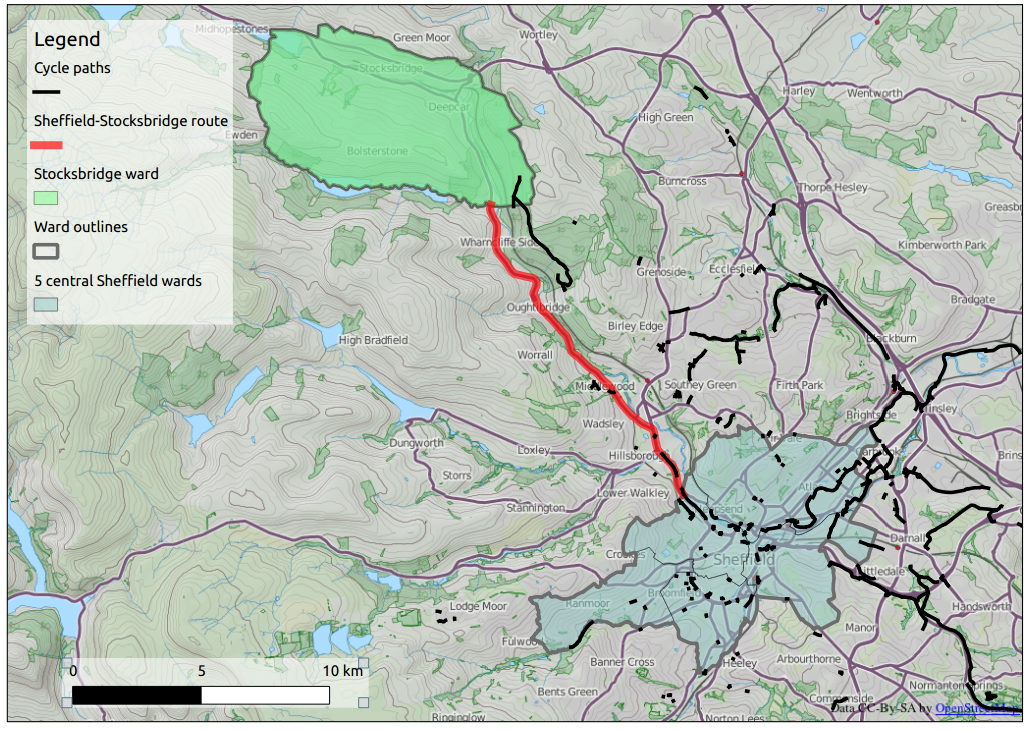
\includegraphics[width = 14 cm]{overview3}}
%     \rule{35em}{0.5pt}
%   \caption{Overview
% of the route between Stocksbridge and Sheffield. }
%   \label{fig:overview3}
% \end{figure}
% 
% Flow data from Nomis at the CAS Ward level provides further
% breakdowns.\footnote{The following figures are quoted to the
% nearest 10 because the flow data has been randomised by
% Nomis to ensure data confidentiality.}
% More than 75\% of these ~2,000 people travel to central Sheffield:
% 1,550 people are reported as working in the five central wards
% (defined as those intersecting with Sheffield's ring road) of
% Broomhill, Burngreave, Castle, Netherthorpe and Sharrow.
% Further breakdowns, by ward, are available: dependence on roads
% is highest for people commuting to Burngreave (explained by
% the lack of a direct bus route to the East of Sheffield from
% Stocksbridge): 98\%. These data are visualised in \cref{fig:stock-mode}.
% 
% \begin{figure}[htbp]
%   \centerline{
%     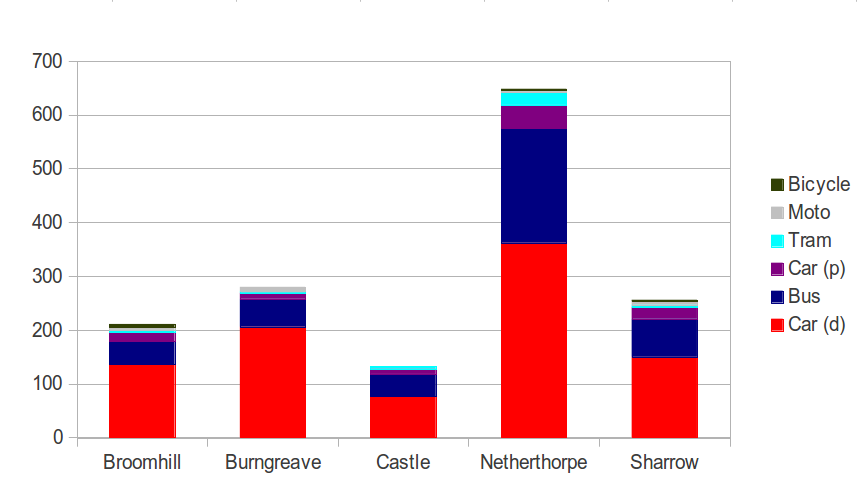
\includegraphics[width = 14 cm]{stock-mode}}
%     \rule{35em}{0.5pt}
%   \caption{Modal split for commutes from
% Stocksbridge to central Sheffield}
%   \label{fig:stock-mode}
% \end{figure}
% 
% \subsection{Defining the scenarios}
% 
% \subsection{Energy savings}
% 
% \subsection{Distributional impacts}
% 
% 
% 
% 
% \subsection{Discussion and conclusions}
% Are the investments worthwhile?

\section{Oil vulnerability} \label{svul}
In addition to greenhouse gas emissions, one of the most problematic features
of modern transport systems in the long term is their high dependence on finite
fossil fuels. This is well illustrated by the fuel tax protests of 2000, when
a small group of protesting hauliers caused chaos in hundreds of petrol
stations in the UK \citep{Lyons2002}.
The high vulnerability of transport systems to relatively minor perturbations
in the supply of oil has not gone unnoticed by the research community.
\citet{McKinnon2006} investigated the impacts of a week-long cessation of
fuel supplies to the UK's road distribution network and arrived at the worrying
conclusion that it would lead rapidly to economic collapse. %y and z !!!
Based on a detailed analysis of the 2008 spike in high prices and subsequent
collapse of the US housing market, \citet{Sexton2011} arrived at the conclusion
that the latter (and much economic strife) was caused by the former, due
primarily to high energy costs of commuting from low density suburbs.

These studies have provided strong evidence that modern transport systems
are highly vulnerable by speculating on possible future outcomes based on
historical precedents. However, few studies have sought to {quantify} the
likely impacts or predict the people and places most likely to be affected.
This section explores methods of measuring `commuter oil vulnerability' based
on spatial microdata of commuters in Yorkshire and the Humber, and generates
results indicating which types of area, and people may most affected by another
oil price spike.


% \subsection{Input data: travel, energy and income} % Removed this section!!!
% A summary of the input data used for the
% vulnerability metrics developed in this paper, the level at which they operate,
% and reasons for their inclusion, are outlined in Table \ref{t:data8}.
% The main data sources available in the UK are taken from the 2001
% Census (at a high geographic resolution) and the Understanding Society
% dataset (USd), an individual level nationwide survey of socio-economic variables
% and attitudes. Clearly, the list of variables affecting oil vulnerability taken
% from these datasets is not comprehensive. Resilience to oil shocks is also
% affected by other variables including level of education,
% community cohesion, strength of the local and regional economy and geographic
% factors such as proximity to farmland and export markets \citep{North2010585,
% Bailey2010}.
% These factors are
% more difficult to quantify, however: data availability precludes their
% inclusion in the model.
% 
% \begin{table}[htbp]
% \caption{Input variables related to vulnerability of commuters to oil shocks}
% \begin{tabular}{p{3cm} p{1.2cm} p{1.8cm} p{1.8cm} p{4cm}}
% 
% Variable & Symbol Units & Dataset & Level & Comments \\ \hline
% Active travel & $P_{act}$ (\%) & Census & Zonal & Baseline of walking/cycling
% \\ \hline
% Car dominance & $P_{car}$ (\%) & Calculated (Census) & Zonal & Dependence on oil
% \\ \hline
% Car sharing & $P_{share}$ (\%)& Census & Zonal & Potential for trip sharing \\
% \hline
% Density & $D{ens}$ ppl/km$^{2}$ & Census & Zonal & Proxy of isolation \\ \hline
% Distance to employment centre & $D_{cent}$ km & Calculated (UKB) & Zonal & Based
% on predefined centres \\ \hline
% Distance to work & $D_{wk}$ km & USd/ Census & Individual & Dependence on
% long-distance travel \\ \hline
% Energy cost of commute & $E_{T}$ MJ/T & USd/ Census & Individual & Calculated
% from distance and mode \\ \hline
% Energy use & $E_{ind}$ MJ/yr & USd & Individual & Proportion of energy budget \\
% \hline
% Energy use & $E_{area}$ MJ/yr & Nstats & Zonal & Relative importance of
% commuting \\ \hline
% Expenditure on commute & $Ex_{T}$ (\pounds/T) & Calculated & Individual &
% Financial vulnerability \\ \hline
% Income & $I$ \hspace{0.5 cm} \pounds/yr & USd & Individual & Financial
% vulnerability \\ \hline
% Infrastructure & $Inf$ km/zone & Ordnance Survey & Zonal & Potential for
% active travel \\
% \hline
% Mode of commute & $M$ \hspace{1 cm}- & USd/ Census & Individual & Fuel
% requirements and expenditure per km \\ \hline
% \end{tabular}
% \label{t:data8}
% \end{table}
% 
% A notable feature of the variables described in Table \ref{t:data8} is that some
% operate at the level of individuals, while others operate at the level of
% geographic zones. This is problematic when developing indices, and necessitates
% methods for combining variables that operate on zonal and individual levels,
% for indices that are `scale independent' \citep{Fotheringham1989} that can apply
% to individuals and zones alike. Of course, for the creation of zonal measures of
% vulnerability, it is possible to aggregate individual variables over
% geographic areas, for example average incomes.
% However, this approach may not be appropriate, for a couple of reasons: first,
% geographic aggregates  ignore the distribution of continuous variables such as
% income; second, certain variables such as income are rarely made
% publicly available for small areas by national governments, for ethical and
% confidentiality reasons \citep{Lee2009}.
% 
% The solution to these problems adopted in this paper is spatial
% microsimulation: a method of allocating individuals to zones based on shared
% variables between individual and geographically aggregated datasets
% (see \citep{Ballas2005b} for overview of method).

% %%% DETAILS ABOUT THE MODEL REMOVED BECAUSE THEY'LL APPEAR IN ANOTHER PAPER
% %zonal and individual level variables (see \citealp{Ballas2005c}).
% % The model
% % selects individuals based on 4 constraints (or `linking variables') which are
% % shared between the individual level Understanding Society dataset (USd) and
% % zonal aggregates from the Census. Importantly, these variables are used to
% % select
% % individuals based on the mode and distance of their trips to work (see  Tables
% % \ref{t:ind} and \ref{t:zone} for sample input data).
% %
% % \begin{table}[htbp]
% % \caption{Sample of linking variables at the individual level (USd)}
% % \begin{tabular}{|r|l|l|r|l|}
% % \hline
% % \multicolumn{1}{|l|}{ID} & Age / sex  & Mode  & \multicolumn{1}{l|}{Distance }
% &
% % NS-SEC  \\ \hline
% % 1 & Male, 59 & Car driver & 3 & lower management \\ \hline
% % 2 & Female, 51 & Car driver & 9 & higher professional \\ \hline
% % 3 & Male, 31 & Car driver & 2 & Other \\ \hline
% % 4 & Female, 24 & Walk & 1 & lower management \\ \hline
% % \end{tabular}
% % \label{t:ind}
% % \end{table}
% %
% % \begin{table}[htbp]
% % \caption{Sample of linking variable values for zones. The population of the
% most
% % populous category is presented for each variable.}
% % \begin{tabular}{|l|r|r|r|r|}
% % \hline
% % Area code & \multicolumn{1}{l|}{Males, 35-54} & \multicolumn{1}{l|}{Car
% drivers}
% % & \multicolumn{1}{l|}{5-10 km} & \multicolumn{1}{l|}{lower management} \\
% \hline
% % E02001509 & 116 & 1616 & 914 & 499 \\ \hline
% % E02001510 & 94 & 1430 & 665 & 402 \\ \hline
% % E02001511 & 82 & 1467 & 848 & 340 \\ \hline
% % E02001512 & 152 & 2280 & 573 & 791 \\ \hline
% % \end{tabular}
% % \label{t:zone}
% % \end{table}
% % % Possible discussion of IPF and integerisation here
% % % The technique used to allocate representative individuals to each zone,
% % % iterative proportional fitting (IPF), results in non-integer weights
% %
% % After processing these input datasets, the output of the spatial
% % microsimulation model is a list of individuals for each zone under
% % investigation. These individuals, taken from the USd, have `target
% % variables' associated with them, such as income, household energy bills and
% % environmental attitudes. These target variables should be viewed not as `real
% % data' but as estimates based on their links to the linking variables at the
% % national level: they are unconstrained by Census data at the aggregate level.
% %
% % By simulating the characteristics of individuals within each geographic area,
% % spatial microsimulation make the variables listed in table
% % \ref{t:data8} available for analysis at individual and zonal levels
% % simultaneously. These variables provide a wide evidence base on which
% % vulnerability indices can be be built. One important variable must be
% % calculated, however: the energy costs of commuting. This data is not provided
% % by Census or survey datasets. It must be calculated, based on existing methods
% % \citep{Fels1975, Lovelace2011-assessing} and available data.

% \subsection{Energy cost data}
% The estimation of energy costs is problematic at the best of times, and
% especially so in the transport sector. Energy use is rarely
% recorded in the `chremastitic' (finance-dominated) economy
% \citep{Martinez-Alier2010} (see \citet{DUKES2011} for an exception).
% Personal transport is especially problematic because vehicles are
% mobile energy consuming devices with
% constantly varying efficiencies \citep{Daly2011}. While heaters and
% electrical appliances use energy from one supplier at a predictable rate,
% cars can be refuelled almost anywhere. Therefore, real world
% energy use datasets are more readily available for electricity
% and heat, the other two major energy users, than for transport
% \citep{MacKay2009}.
% % % \footnote{Gas and electricity use
% % % are monitored down to the level of Lower Super Output Areas, (LSOAs,
% % % each containing \~ 1,500 citizens), and expenditure (from which energy usage
% % % can be deduced) on domestic energy bills are provided at the household level
% % by
% % % a number of national surveys.}
% 
% Vehicle emissions (and hence energy use) can be estimated based on
% traffic flow data provided by the Department for Transport (DfT),\footnote{See
% the publicly available Inter-Urban Congestion Dataset:
% http://data.gov.uk/dataset/dft-eng-srn-routes-journey-times}
% sales data from petrol stations (where data is available), and inference from
% transport to work statistics. The third option is used here, as data is
% available for its estimation (Table \ref{t:e}), and commuting behaviour is
% well-constrained, at local levels, by the Census.
% 
% \vspace{5cm}
% 
% \begin{table}[h]
% \caption[Direct energy use and occupancy by mode]
% {Direct energy use and average occupancies of for the 7 most frequently
% used modes of commuting.}\centering{
% \begin{tabular}{lrrrr}
% {Mode} & \multicolumn{1}{l}{Ef (MJ/vkm)} &
% \multicolumn{1}{l}{Occupancy} &
% \multicolumn{1}{l}{EI (MJ/pkm)} &
% \multicolumn{1}{l}{Distance (km)$^g$} \\ \hline
% Bicycle & 0.093$^a$ & 1& 0.09 & 4.4 \\
% Bus & 7.34$^b$ & 9$^b$ & 0.82 & 8.3 \\
% Car & 2.98$^c$ & 1.186$^d$ & 2.40 & 15.2 \\
% Metro & -- $^e$  & 1$^*$ & 0.54 & 9.4 \\
% Motorbike & 1.87$^f$ & 1.16$^f$ & 1.61 &  10.6\\
% Train & 63.4$^b$ & 182$^b$ & 0.35 & 37.2 \\
% Walking & 0.13$^a$ & 1 & 0.13 & 1.3 \\
% \end{tabular}}
% \label{t:e}
% \end{table}
% \begin{footnotesize}
%  a: \citet{Coley2002}, b: \citep{Hansard2005}, b:
% \citet{Treloar2004}, c:
% \citet{MacKay2009}, d: \citet{DfT2011-commuting}, e:
% \citet{LondonUnderground2007}, f: \citet{ORNL2011}, g: Calculated from
% \citet[Table 4]{DfT2011-commuting}, *: Data provided per person kilometre.
% \end{footnotesize}

% % \subsection{Economic data}
% %
% % Following UK and EU government recommendations for measuring poverty and fuel
% % poverty \citep{Fahmy2011}, `equivalised' income was used as the
% % denominator for calculating commuter vulnerability based on proportion of
% income
% % spent on travel to work \citep{Moore2012}. The much-cited OECD equivalisation
% % method \citep{OECD} was used to calculate equivalised income, based on
% household
% % income (question xxx) and number of adult and child inhabitants (xxx) provided
% % by the USd.

\subsection{Metrics of vulnerability: resources, jobs, money}
\label{metrics}
Four metrics, which reflect economic, energetic and other
perspectives on oil vulnerability, were developed, and calculated
for zones in Yorkshire and the Humber. The inputs into the vulnerability
metrics were supplied by the results of the spatial microsimulation model.
These metrics are as follows:
\begin{itemize}
 \item Economic vulnerability: defined as commuter fuel poverty ($V_{cfp}$),
the proportion of people spending more
than 10\% of their income on work travel.
\item Energy based metric 1: proportion of energy use expended on
work travel ($V_e$)
\item Energy based metric 2: proportion of individuals
spending more than 10\% of their `energy
budget' on work travel in each area ($V_{ei}$).
\item Hybrid vulnerability index based on distance to employment centre,
dominance of cars, and the average energy costs of commute ($V_h$).
\end{itemize}

% %%%%% This is more like discussion, so removed for now.
% % The scarcity of suitable energy resources lies at the root of commuter
% % vulnerability to high oil prices. However, it is the monetary manifestation of
% % this scarcity --- high fuel prices --- that currently leads to suffering at
% % household and
% % family levels, according to recent evidence. During the oil price
% % shock of 2008, these financial impacts put unprecedented pressure on
% low-income
% % suburban commuters in the USA, leading to an increase
% % of mortgage defaults and as commuting became unaffordable \citet{Sexton2011}.
% %
% % From these foreclosures result social costs, including stress,
% % dislocation from the local community (when households are forced out of their
% % homes), poor health and in some cases divorce \citep{Libman2012}. These
% % indirect economic impacts are what do the damage, rather than the abstract
% % impact of ``using a high proportion of one's daily energy use on
% % commuting''. Clearly the two are related, but it seems scarcity of money is
% the
% % most tangible end result. Ecological economists may counter that, in the long
% % term and at the system level, energy is more important than money
% % \citep{Odum2006}.
% % For this reason
It should be noted that two of these metrics, $V_{cfp}$ and $V_e$, also
operate at the individual level, allowing for the identification of
characteristics associated with vulnerability to be assessed in each zone
(see Section \ref{s:indresults}).
Both financial and energy metrics of commuter vulnerability are
used. The former has strong foundations in economics; the latter in systems
ecology. Finally, a more complex hybrid vulnerability metric is presented.

\subsubsection{Economic vulnerability --- commuter fuel poverty}
The total monetary costs per trip ($C$) can be estimated as a function of the
value of time lost ($c_s$) and direct monetary expenditure ($c_m$) per unit
distance ($d$) for each mode of transport \citep{Ommeren2006}. Due to
methodological difficulties in measuring $c_s$ \citep{Mokhtarian2001}, we
focus on the the direct monetary costs:

\begin{equation}
 C = c_m \times d
\end{equation}

The standard definition of fuel poverty is spending more than 10\% of
disposable household income --- specifically, equivalised income --- on
adequate home heating and cooking \citep{Boardman2010}. Thus,
`commuter fuel poverty' can be defined as spending more than 10\% of one's
equivalised income on commuting. At the individual level, commuter
vulnerability can thus be defined either as a continuous
($V_{cfp}$, equation \ref{e:cfpc}), or a binary ($V_{cfp}bin$, equation
\ref{e:cfpb}) variable.
% the latter determining if they are `commuter fuel poor', or not.
For zones, vulnerability can be defined simply as the proportion of people
living in  commuter fuel poverty ($V_{cfp}a$, \ref{e:cfp}). %, for whom $C/I >
\begin{equation}
 V_{cfp} = C/I
\label{e:cfpc}
\end{equation}

\begin{subnumcases}{V_{cfp}bin=}
1, & if $V_{cfp} \geq 0.1$ \\
0, & if $V_{cfp} < 0.1$
\label{e:cfpb}
\end{subnumcases}

\begin{equation}
 V_{cfp}a = \frac{\sum V_{cfp}bin}{n}
\label{e:cfp}
\end{equation}

\subsubsection{Energy-based metrics}
An alternative approach is to take the ecological view that energy is the
`master resource' \citep{Smil2006}, and measure vulnerability
accordingly.\footnote{According to this view, a system's
performance can be assessed by the energy flows within it \citep{Odum1971}}.
The resulting metric would focus not on the monetary expenditure of transport
to work, but on the energy costs. Using the data presented in \cref{Chapter5},
energy costs per trip ($E_T$) can be calculated based on information on mode
($_m$), distance ($d$), and energy consumption per kilometre ($\eta$):

\begin{equation}
 E_T = \eta_m \times d
\label{e:e}
\end{equation}

This estimate can be used as a self-standing marker of vulnerability, if one
assumes that more energy intensive commuting patterns are
inherently more vulnerable. Following the logic of fuel poverty measures,
an alternative to monitoring absolute energy use in transport is
 the \emph{proportion} of one's energy budget expended on commuting ($P_{ET}$):

\begin{equation}
P_{ET} = \frac{E_T \times T_{yr}}{E_{yr}}
\label{e:pet}
\end{equation}
where $T_{yr}$ is the number of commuter trips made per year and $E_{yr}$ is
total energy use per year. These input values can be calculated at the
individual level from the survey data.
At the individual level, the resulting energy-based vulnerability metrics
($V_{ei}$) can therefore be calculated as continuous or binary individual level
variables. For geographic zones, $V_{ei}$ is defined as the proportion of
commuters who spend more than 10\% of their energy budget on work travel.

An alternative energy-based vulnerability metric that operates solely at the
aggregate level ($V_e$) is calculated as the total energy expenditure on
commuting in the area divided by total domestic energy use:

\begin{equation}
 V_e = \frac{ \sum E_T \times T_{yr}} {\sum E_{yr}}
\end{equation}

\subsubsection{Hybrid vulnerability metrics}
A criticism of the aforementioned vulnerability indexes is their narrow focus,
either on energy or money. They take no account of other quantifiable factors
that influence vulnerability, such as geographical isolation from employment
centres, level of community cohesion or the diversity of transport
options in the area \citep{Pickerill2008,
North2010585, Steele2010mind, newman2009resilient}.
For this reason, a hybrid metric based on multiple risk
factors may be more appropriate. The following is one example of a hybrid
index that operates at the aggregate level:

\begin{equation}
 V_h = (P_{ET} + \alpha) \times \sqrt{\beta D_{c}} \times P_{car}
\label{e:ev}
\end{equation}
where $P_{ET}$ is the proportion of the individual's energy budget spent on
commuting, $D_{c}$ is distance to employment centre, $P_{car}$ is the proportion
of work trips made by car in the zone in question, and $\alpha$ and $\beta$ are
parameters to be set.

$V_h$ acknowledges that the vulnerability of commuting patterns to high oil
prices is complex, and caused by multiple, self reinforcing factors. By
changing the values of the predefined parameters (or by modifying the equation)
it is possible to increase or decrease the importance allocated to certain
factors. Increasing the value of $\alpha$, for example makes the result far less
sensitive to the proportion of energy used for commuting. Perhaps isolation is
seen as a more important determinant. In this case the value of $\beta$ could
be increased.\footnote{This
assumes that $D_{c}$ is a valid proxy for isolation.
Whether or not the assumption holds is debatable, based on the method used to
calculate $D_{c}$ for each zone: $D_{c}$ is defined here as the
distance to the nearest employment centre in each
transport to work (TTW) zone.  $D_{c}$ was  calculated for the
population centroid of each medium super output area (MSOA) using
the command `nncross' from the `spatstat' package in the computer program R.
}


% % A problem with both the monetary and energetic metrics is that they do not
% take
% % into account the advantages of proximity to employment centres. Whether or not
% % these employment
% % centres will provide an adequate number of jobs in an energy scarce future is,
% % of course, open to debate \citep{Greer2009}. Our models inherently contain
% % assumptions about the future \citep{Smil1993}. According to the previous
% % metrics, the trip to work is constant for people over time and do not depend
% on
% % geographical location. However, this is clearly not the case: people change
% % jobs for travel reasons, and also change the mode of transport to work. As
% % illustrated in Fig.~\ref{fig:dis-e}, many people in living in city centres
% % travel a long way to work. This can be interpreted as follows: local
% % employment opportunities exist in the employment centre, but highly qualified
% % and wealthy people choose to travel further afield for work. Thus, although
% % these individuals may spend a high proportion of their monetary and energy
% % budgets on commuting, they are not as vulnerable to high oil prices as these
% % static metrics would imply: if oil prices increase, they could likely find
% work
% % in the local area. Therefore, the final metric of commuter vulnerability takes
% % distance into account, yet retains the focus on economic rather than energetic
% % performance:
% 
% 
% % The vulnerability of commuters to high oil prices is therefore be defined as
% % the proportion of their income that is spent on the \emph{fuel} costs of
% % commuting. The distinction between fuel costs and total commuting costs is
% % important: while train travel may be unaffordable, its price is not vulnerable
% % to unpredictable fluctuations in the international price of oil. Car travel,
% by
% % contrast is. This is captured in estimates of the direct liquid fuel
% % requirements of each mode of transport. Multiplying by the price of fuel (at
% % the pump) results in the monetary expenditure on fuel required by each form of
% % transport (Table x).

Each of these metrics has its limitations, not least the reliance on aggregate
cost and energy estimates that may vary significantly from place to place and
person to person. These limitations are further discussed in Section
\ref{discuss}.
For now the assumption is that they are useful proxies of commuter
oil vulnerability and, after exploring aggregate level
findings based on census data, investigate the results of each formulae in turn.

% \subsection{A spatial microsimulation model of commuter patterns}
% \label{s:msim}
% The data and equations presented above can operate at regional and
% individual levels: as zonal averages supplied by the Census or individual cases
% supplied by Understanding Society. Both have advantages. Regional data from the
% Census (supplied by the Casweb data portal) illustrate the spatial
% patterns in commuting behaviour, but
% mask variation at the individual level \citep{Openshaw1983}. Individual level
% data illustrate the inequalities that exist between people, and the links
% between commuting and other individual level variables such as income,
% socio-economic class and qualifications. Survey data are not geocoded, however.
% 
% Spatial microsimulation combines `the best of both worlds' by
% allocating individual microdata to zones based on shared variables between
% survey (individual level) and census (regional) data \citep{Ballas2005b}. The
% linking variables used for this microsimulation model were age, sex, mode of
% transport to work, distance of commute and socio-economic class. Iterative
% proportional fitting (IPF) was used to reweight the survey dataset for each
% medium super output area (MSOA)
% zone in Yorkshire and the Humber. Because individuals from the
% Understanding Society dataset are selected, simulated values for a range of
% other variables can be made, including income, work times (and therefore
% frequency of the trip made to work over the year) and domestic energy use (gas
% and electricity bills).

\subsection{Results: trips, distance and energy use}
\label{results8}
% \begin{table}[h]
% \caption{Summary statistics of typical commuter patterns and energy use for
% MSOA zones in Yorkshire and the Humber.}
% \begin{tabular}{lrrrrr}
%
% Mode & \multicolumn{1}{l}{N} & \multicolumn{1}{l}{D (km)}
% & \multicolumn{1}{l}{D/T (km)} & \multicolumn{1}{l}{Energy costs (MJ)} &
% \multicolumn{1}{l}{Energy/T (MJ)} \\ \hline
% Bike & 90 & 386 & 4.3 & 69 & 0.8 \\
% Bus & 318 & 2076 & 6.5 & 3404 & 10.7 \\
% Car & 1716 & 26376 & 15.4 & 157203 & 91.6 \\
% Carp & 222 & 3113 & 14.0 & 0 & 0.0 \\
% Metro & 12 & 113 & 9.4 & 122 & 10.2 \\
% MFH & 348 & 0 & 0.0 & 0 & 0.0 \\
% Moto & 29 & 306 & 10.6 & 709 & 24.4 \\
% Train & 48 & 1226 & 25.5 & 858 & 17.9 \\
% Walk & 332 & 1013 & 3.1 & 263 & 0.8 \\ \hline
% Total & 3115 & 34609 & \multicolumn{1}{l}{-} & 162628 & \multicolumn{1}{l}{-}
% \\
% \end{tabular}
% \label{}
% \end{table}

The spatial microsimulation model allows
cross-tabulations of commuter patterns by a range of variables.
Table \ref{t:props} illustrates the importance of
the three most popular modes in terms of fundamental features: proportion of
trips,
distance, and energy use.
% \footnote{Note that these results
% apply to Yorkshire and the Humber overall, and mask local variation:
% in a handful of MSOA areas car drivers account for
% less than a third of all commuter trips.}
The dominance of the car is striking. Drivers
(excluding car passengers) account for
55\% of trips, 75\% of distance travelled and
96\% of energy use. This result is predictable as the region's
transport infrastructure is focussed on the
car, and coincides with other findings from the UK
\citep{Brand2013}.\footnote{Yorkshire
and the Humber's transport infrastructure contains 380 km
of motorways, 2,300 km of major roads and over 30,000 km of roads in total.
By contrast there are 1,500 km of railways and less than 500 km of
bicycle paths in the region.}
Overall, cars consume more than 20 times more energy than all other
forms of transport to work put together whilst providing transport for
62\% of the workers.

\begin{table}[htbp]
\caption[Proportion of trips (T), distance (D) and energy (E)
by mode]{Proportion of trips (T), distance (D) and energy (E)
used by the three most
popular forms of transport in Yorkshire and the Humber.}
\begin{center}
\begin{tabular}{lrrr|rrr|rrr|rrr}
\toprule
Dis. & \multicolumn{ 3}{c}{Car*} & \multicolumn{ 3}{c}{Walk} & \multicolumn{
3}{c}{Bus} & \multicolumn{ 3}{c}{All modes} \\
(km) & \multicolumn{1}{l}{T} & \multicolumn{1}{l}{D} & \multicolumn{1}{l}{E} &
\multicolumn{1}{l}{T} & \multicolumn{1}{l}{D} & \multicolumn{1}{l}{E} &
\multicolumn{1}{l}{T} &
\multicolumn{1}{l}{D} & \multicolumn{1}{l}{E} & \multicolumn{1}{l}{T} &
\multicolumn{1}{l}{D} & \multicolumn{1}{l}{E} \\ \midrule
0-2 & 1.2 & 0.1 & 0.2 & 3.5 & 0.4 & 0.0 & 0.2 & 0.0 & 0.0 & 16.8 & 0.6 & 0.2 \\
2-5 & 12.8 & 3.8 & 4.9 & 5.9 & 1.4 & 0.1 & 4.8 & 1.5 & 0.5 & 28.3 & 8.1 & 5.6 \\
5-10 & 15.5 & 10.4 & 13.4 & 0.4 & 0.3 & 0.0 & 3.8 & 2.5 & 0.9 & 23.4 & 15.7 &
14.6 \\
10-20 & 14.0 & 17.3 & 22.2 & 0.7 & 0.8 & 0.0 & 0.9 & 1.1 & 0.4 & 17.7 & 21.7 &
23.0 \\
20-50 & 7.9 & 21.1 & 27.0 & 0.0 & 0.0 & 0.0 & 0.3 & 0.8 & 0.3 & 10.0 & 26.5 &
27.7 \\
50+ & 3.0 & 22.3 & 28.6 & 0.0 & 0.0 & 0.0 & 0.0 & 0.0 & 0.0 & 3.8 & 27.5 & 28.8
\\
All & 54.6 & 75.0 & 96.4 & 10.6 & 2.9 & 0.2 & 10.1 & 5.9 & 2.1 & 100 & 100 & 100
\\ \bottomrule
\end{tabular}\end{center}
\label{t:props}
{\footnotesize *Excludes car passengers}
\end{table}

An additional inequality surrounds distance: trips of more than 10 km account
for
76\% of the distance travelled and 80\% of the energy costs of transport to
work,
yet are made by just 31\% of employees. The results suggest that very long trips
to work consume a disproportionate amount of energy: 4\% of commutes in
Yorkshire and
the Humber are greater than 50 km, yet these account for almost 30\% of energy
costs.

% \subsubsection{The geography of vulnerability}

% % \begin{figure}[h]
% %  \centering
% %  \includegraphics[width=14 cm]{dismap-ms}
% %  % Graph-line.pdf: 516x363 pixel, 72dpi, 18.20x12.81 cm, bb=0 0 516 363
% %  \caption{Average distance travelled to work in Yorkshire and the Humber by
% MSOA
% % zone.}
% %  \label{fig:map1}
% % \end{figure}
% 
% % From Fig.~\ref{fig:map1} it is clear that there is a strong link between
% % geographic location and distance travelled to work. MSOA areas located in and
% % around the conurbations surrounding Bradford, Sheffield and Hull tend to have
% % low average commuter distances, while rural locations such as the North
% % Yorkshire moors are associated with long average commutes.
% % This result differs
% % from that of suburban USA (where urban sprawl accounts for high commuting
% costs
% % even within major conurbations), but it is hardly new or surprising. The
% % influence of the road network on commuter distances is not clear from the map.
The spatial variability of the vulnerability indices is shown in
Fig.~\ref{fig:ve}.
The metrics are closely related, as illustrated by the concentration of
high vulnerability in isolated rural areas in all but one of the metrics.
Spatially this correspondence can be seen as an arc of vulnerable areas
defined in terms of $V_{cfp}$, $V_e$ and $V_h$ in Fig.~\ref{fig:ve}.  This
area runs from East Leeds to Castleford Selby and north-east towards Hull and
the Yorkshire Wolds.
The correlation between the metrics, at the MSOA level, is shown in
Fig.~\ref{fig:scat-mat}.

% % Possible explanatory factors may be the motorways, lack of employment centres
% the area,
% % being former coal mining country [so run down ex-pit villages where people
% travel elsewhere to work].

\begin{figure}[pth]
 \centering
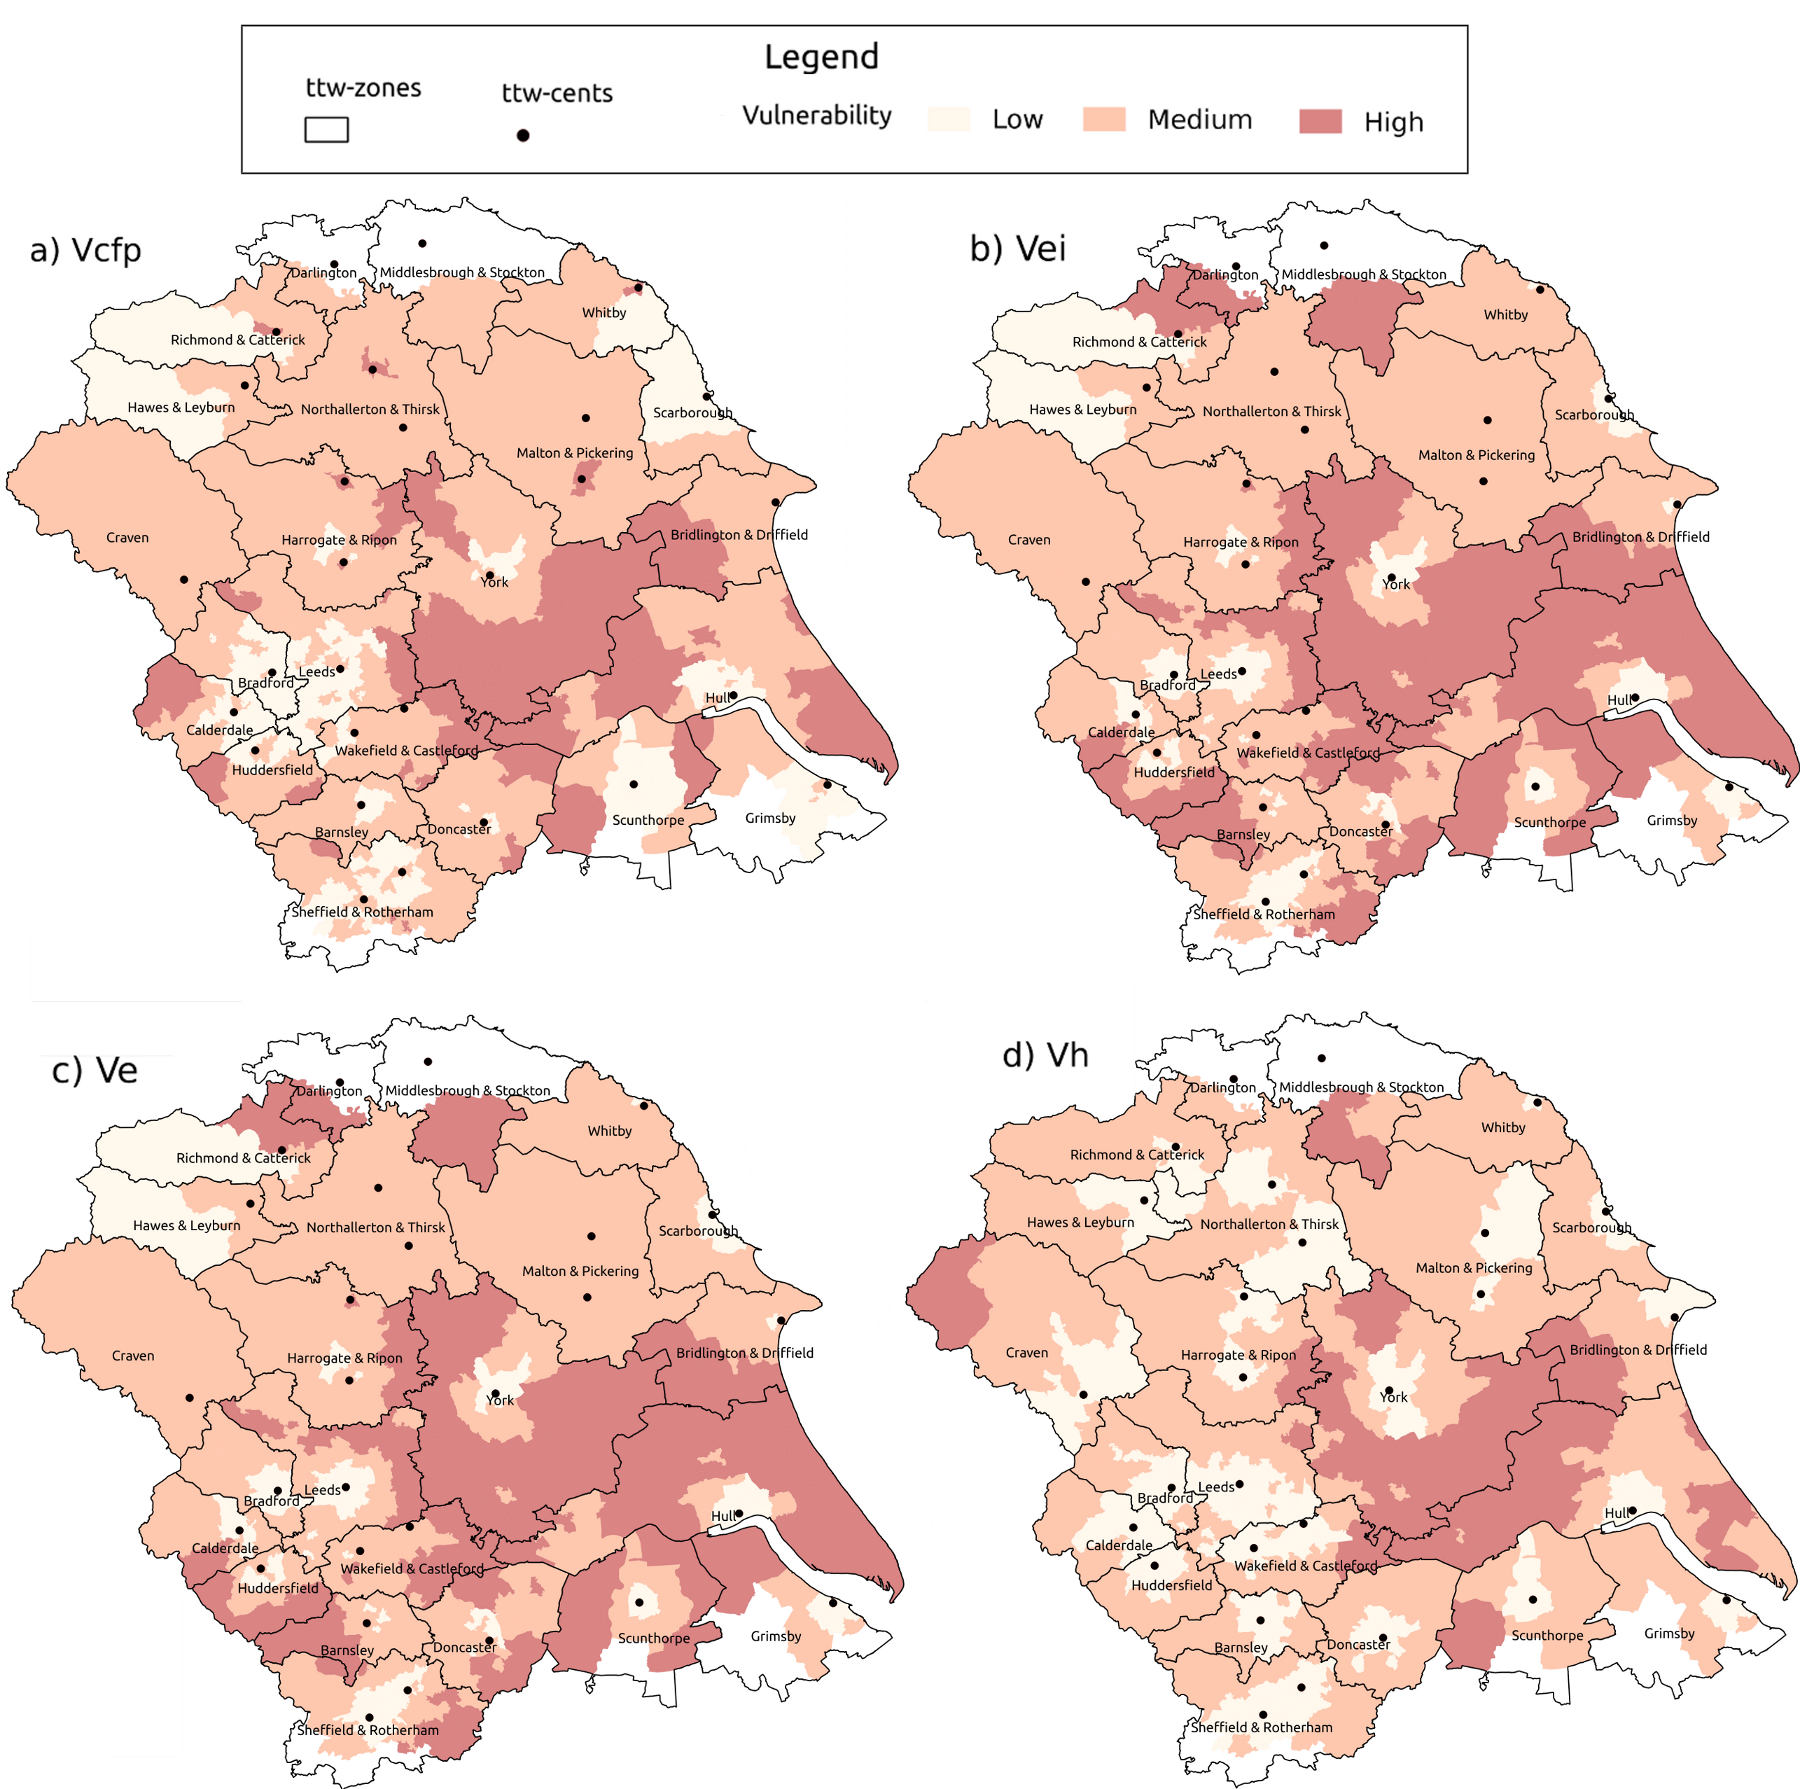
\includegraphics[width=13cm]{vall2}
 % Graph-line.pdf: 516x363 pixel, 72dpi, 18.20x12.81 cm, bb=0 0 516 363
 \caption[Vulnerability of commuter patterns in Yorkshire and the Humber]
 {Vulnerability of commuter patterns in Yorkshire and the Humber
according to four metrics: a) Commuter fuel poverty, b) individual
energetic, c) zonal energetic, d) hybrid vulnerability. Bins
were allocated by Jenks' classification of natural breaks.}
 \label{fig:ve}
\end{figure}

An unexpected result is that some employment centres are associated
with high levels of commuter fuel poverty --- measure a).
This can be seen in the dark patches next to Harrogate, Malton and Whitby
and a number of urban settlements --- for example to the East of Sheffield.
This result can be explained by distance of commute: each of the areas mentioned
is associated with long commutes\footnote{The average Euclidean distances
of commutes in the area are 18, 15 and 23 km for MSOA areas surrounding
Horrogate, Malton and Whitby, respectively. The average for the region
is 11 km.}  and low levels of deprivation
scores in the surrounding areas.

\begin{figure}[t]
 \centering
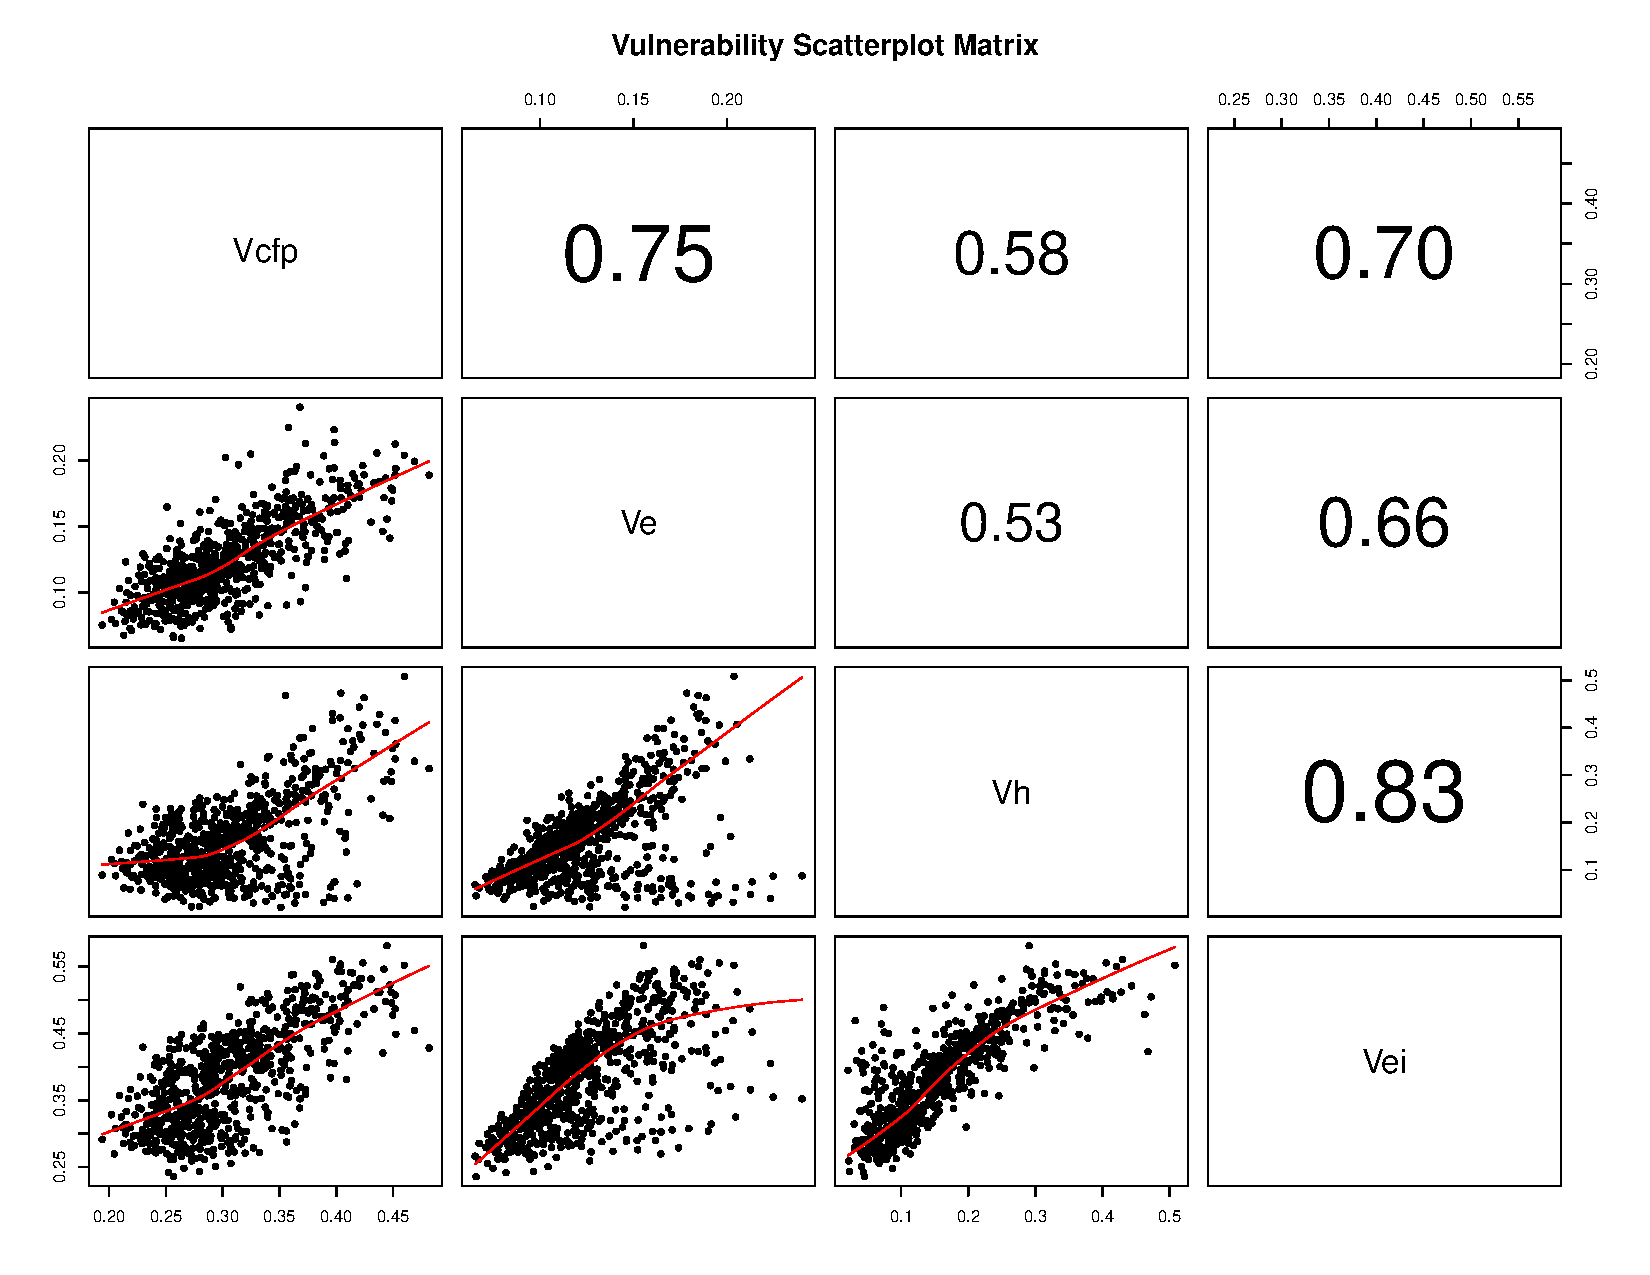
\includegraphics[width=13cm]{scat-mat.pdf}
 % Graph-line.pdf: 516x363 pixel, 72dpi, 18.20x12.81 cm, bb=0 0 516 363
 \caption[Scatterplot matrix of vulnerability metrics]
 {Scatterplot matrix illustrating the relationships between each of
the 4 vulnerability metrics.}
 \label{fig:scat-mat}
\end{figure}

In order to test the relationship between commuter oil vulnerability and
broader social disadvantage, the vulnerability measures were compared
with the Index of Multiple Deprivation (IMD). Because IMD data is available
at the lower super output area (LSOA), aggregation was used to find the mean
IMD score in each MSOA. This allowed correlations to be calculated.
Negative correlations were found between aggregated IMD and
all four vulnerability metrics;
Pearson's coefficient of correlation
(r) ranged from -0.59 to -0.22
for the $V_{ei}$ and $V{cfp}$ measures respectively.
This result implies that
areas at risk from high oil prices are not currently identified as
being in urgent need of support. A comparison of the chloropleth maps
of IMD in Fig.~\ref{fig:IMD} with the vulnerability metrics
(Fig.~\ref{fig:ve}) illustrates the reason
for negative correlations: deprivation is primarily a urban phenomenon in
Yorkshire and the Humber (the three most deprived MSOA areas
are located near central Grimsby and Hull),
whereas oil vulnerability tends to be rural.

\begin{figure}[t]
 \centering
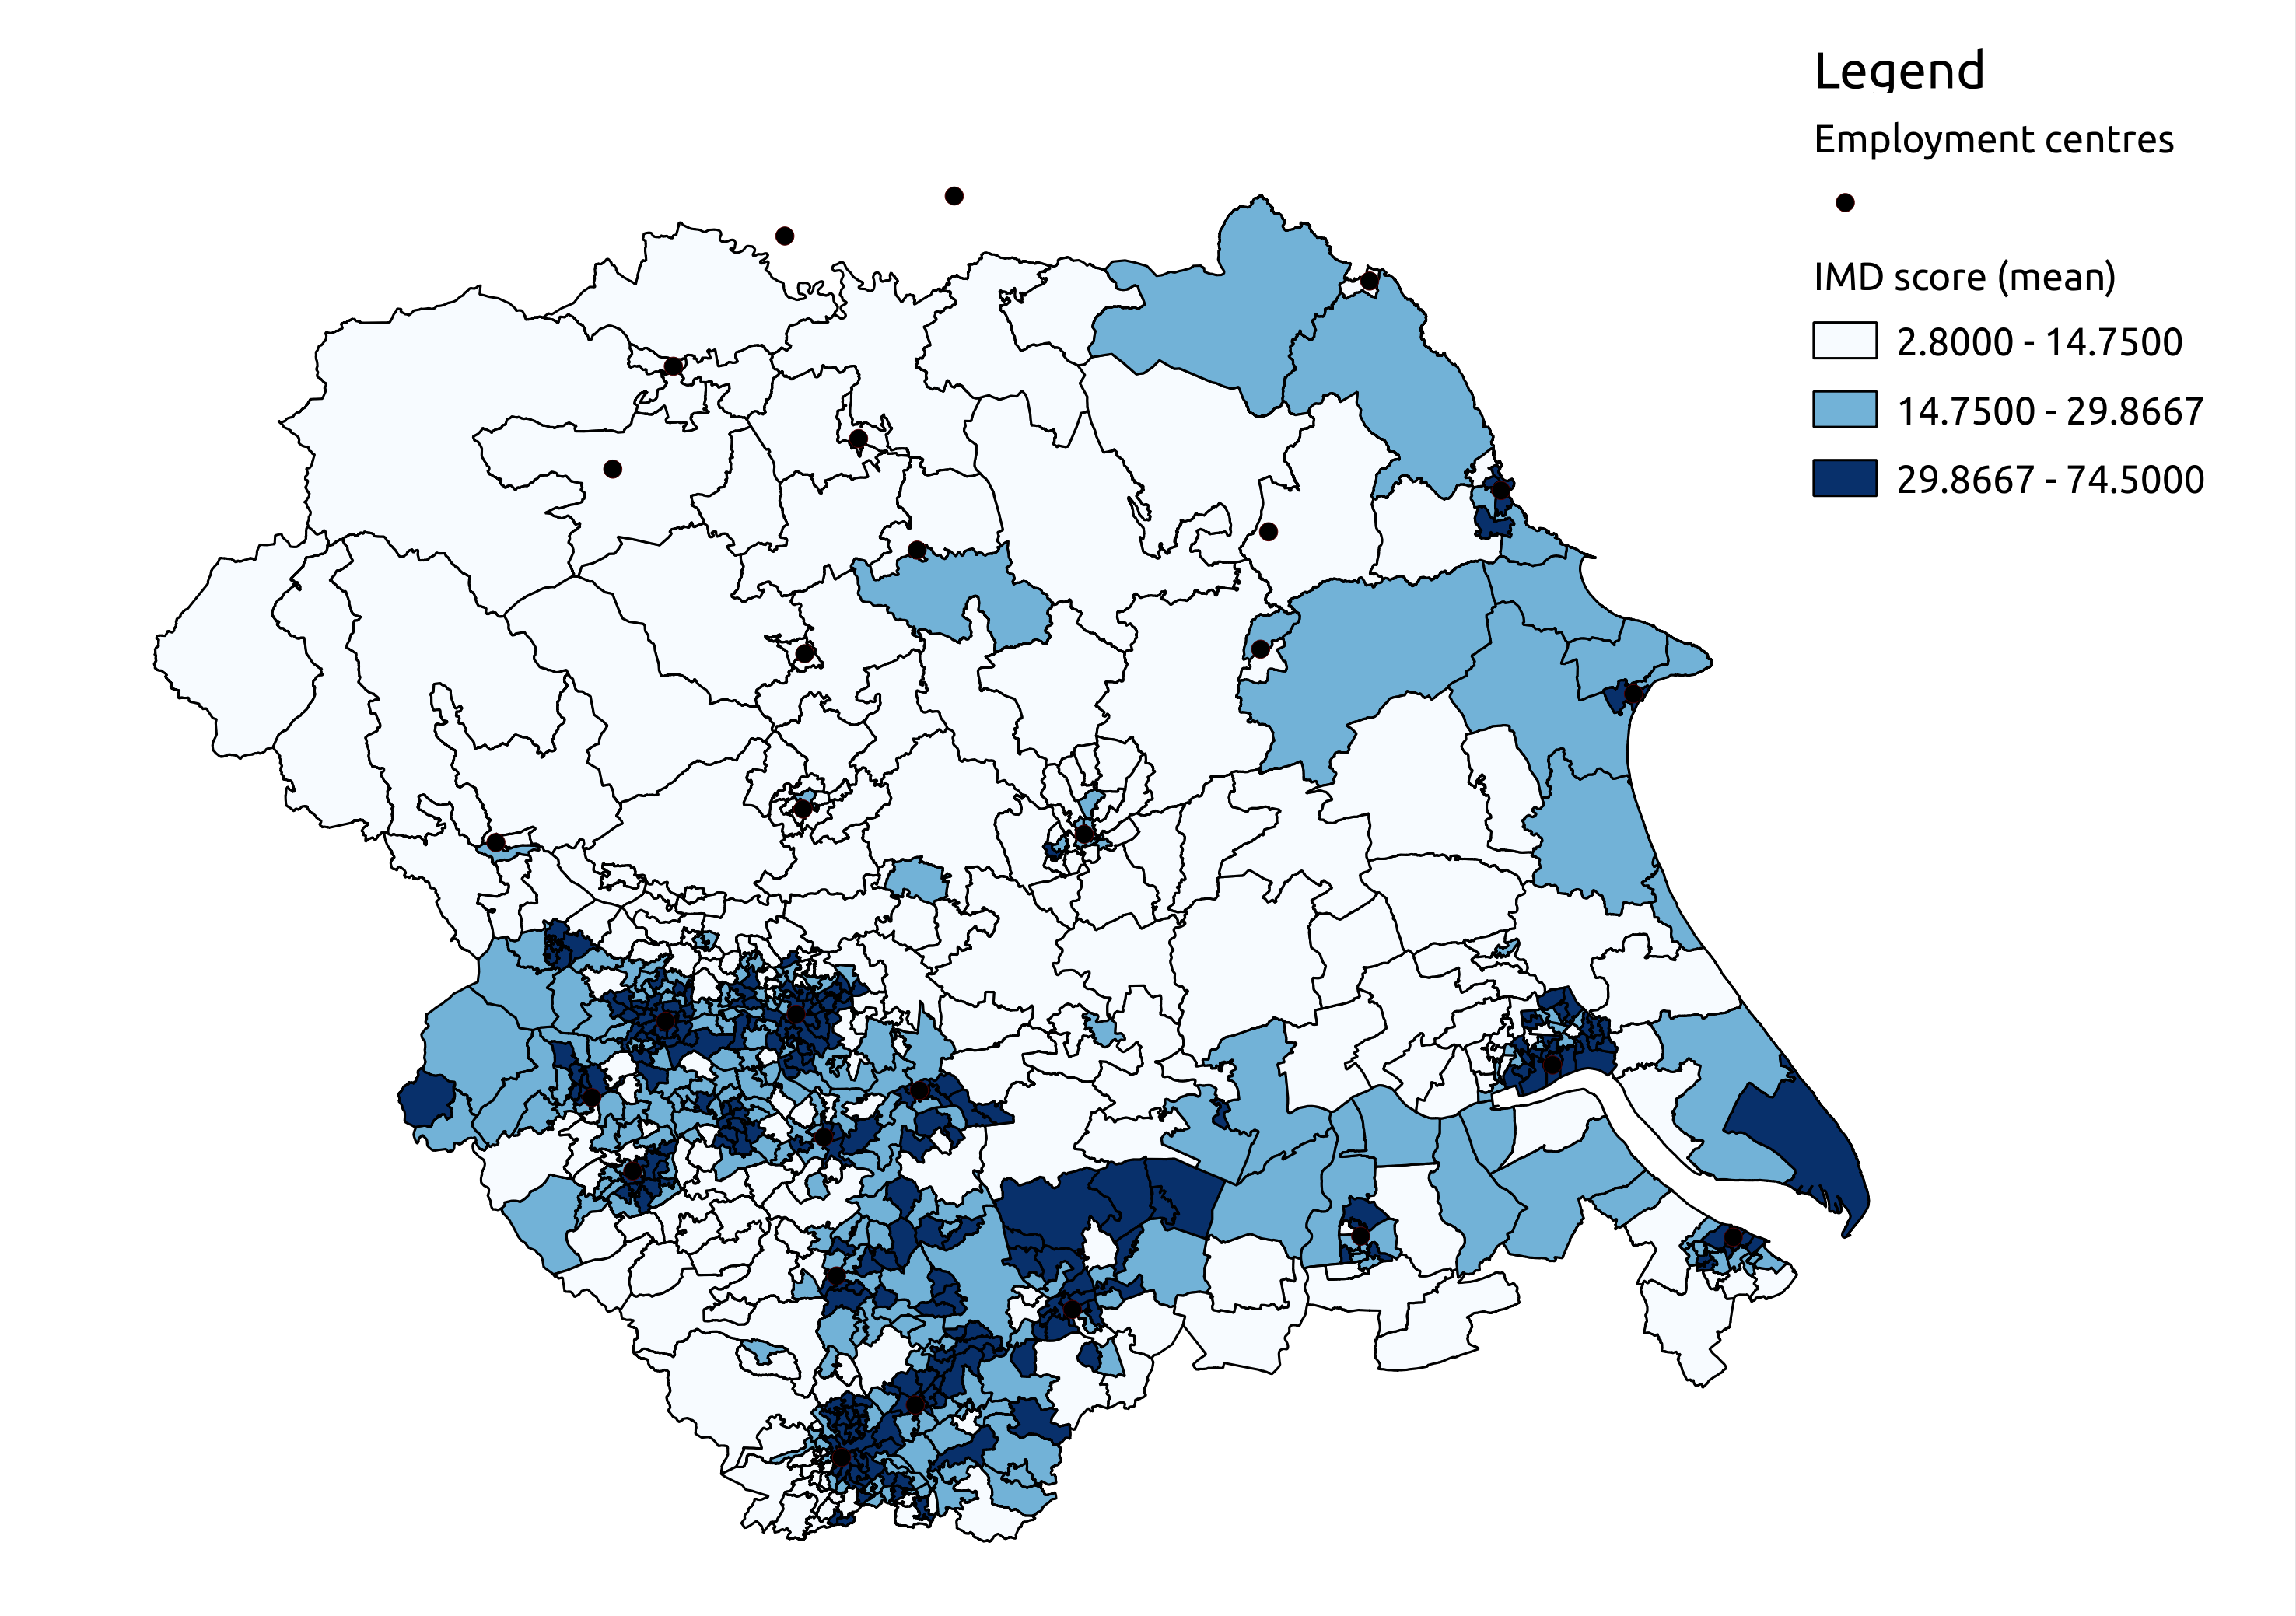
\includegraphics[width=13cm]{IMD}
 % Graph-line.pdf: 516x363 pixel, 72dpi, 18.20x12.81 cm, bb=0 0 516 363
 \caption[Chloropleth map of deprivation in Yorkshire and the Humber]
 {Chloropleth map illustrating the spatial variability of
the Index of Multiple Deprivation at the MSOA level. (Values are
average IMD scores for LSOA centroids.)}
 \label{fig:IMD}
\end{figure}

To explore this link further, the average distance from employment
centre\footnote{``Employment centre'' here is defined as the towns and cities
referred to in the names of the 2001 transport to work areas (TTW)
\citep{ONS2011-ttw}.} was calculated, based on the population-weighted centroids
of the MSOA areas and the economic centre of each transport to work area, based
on 2001 data. The results (illustrated in Fig.~\ref{fig:mapttw}) demonstrate
the importance of taking account of population clustering in the analysis of
zones: population-weighted centroids are often much closer to employment
centres than centroids that are based on area alone.
The similarities between
the metrics plotted in Fig.~\ref{fig:ve}
and the distance from employment centre illustrated in Fig.~\ref{fig:mapttw}
suggest a strong link between distance from employment hub, energy use, and
vulnerability.

\begin{figure}[h]
 \centering
   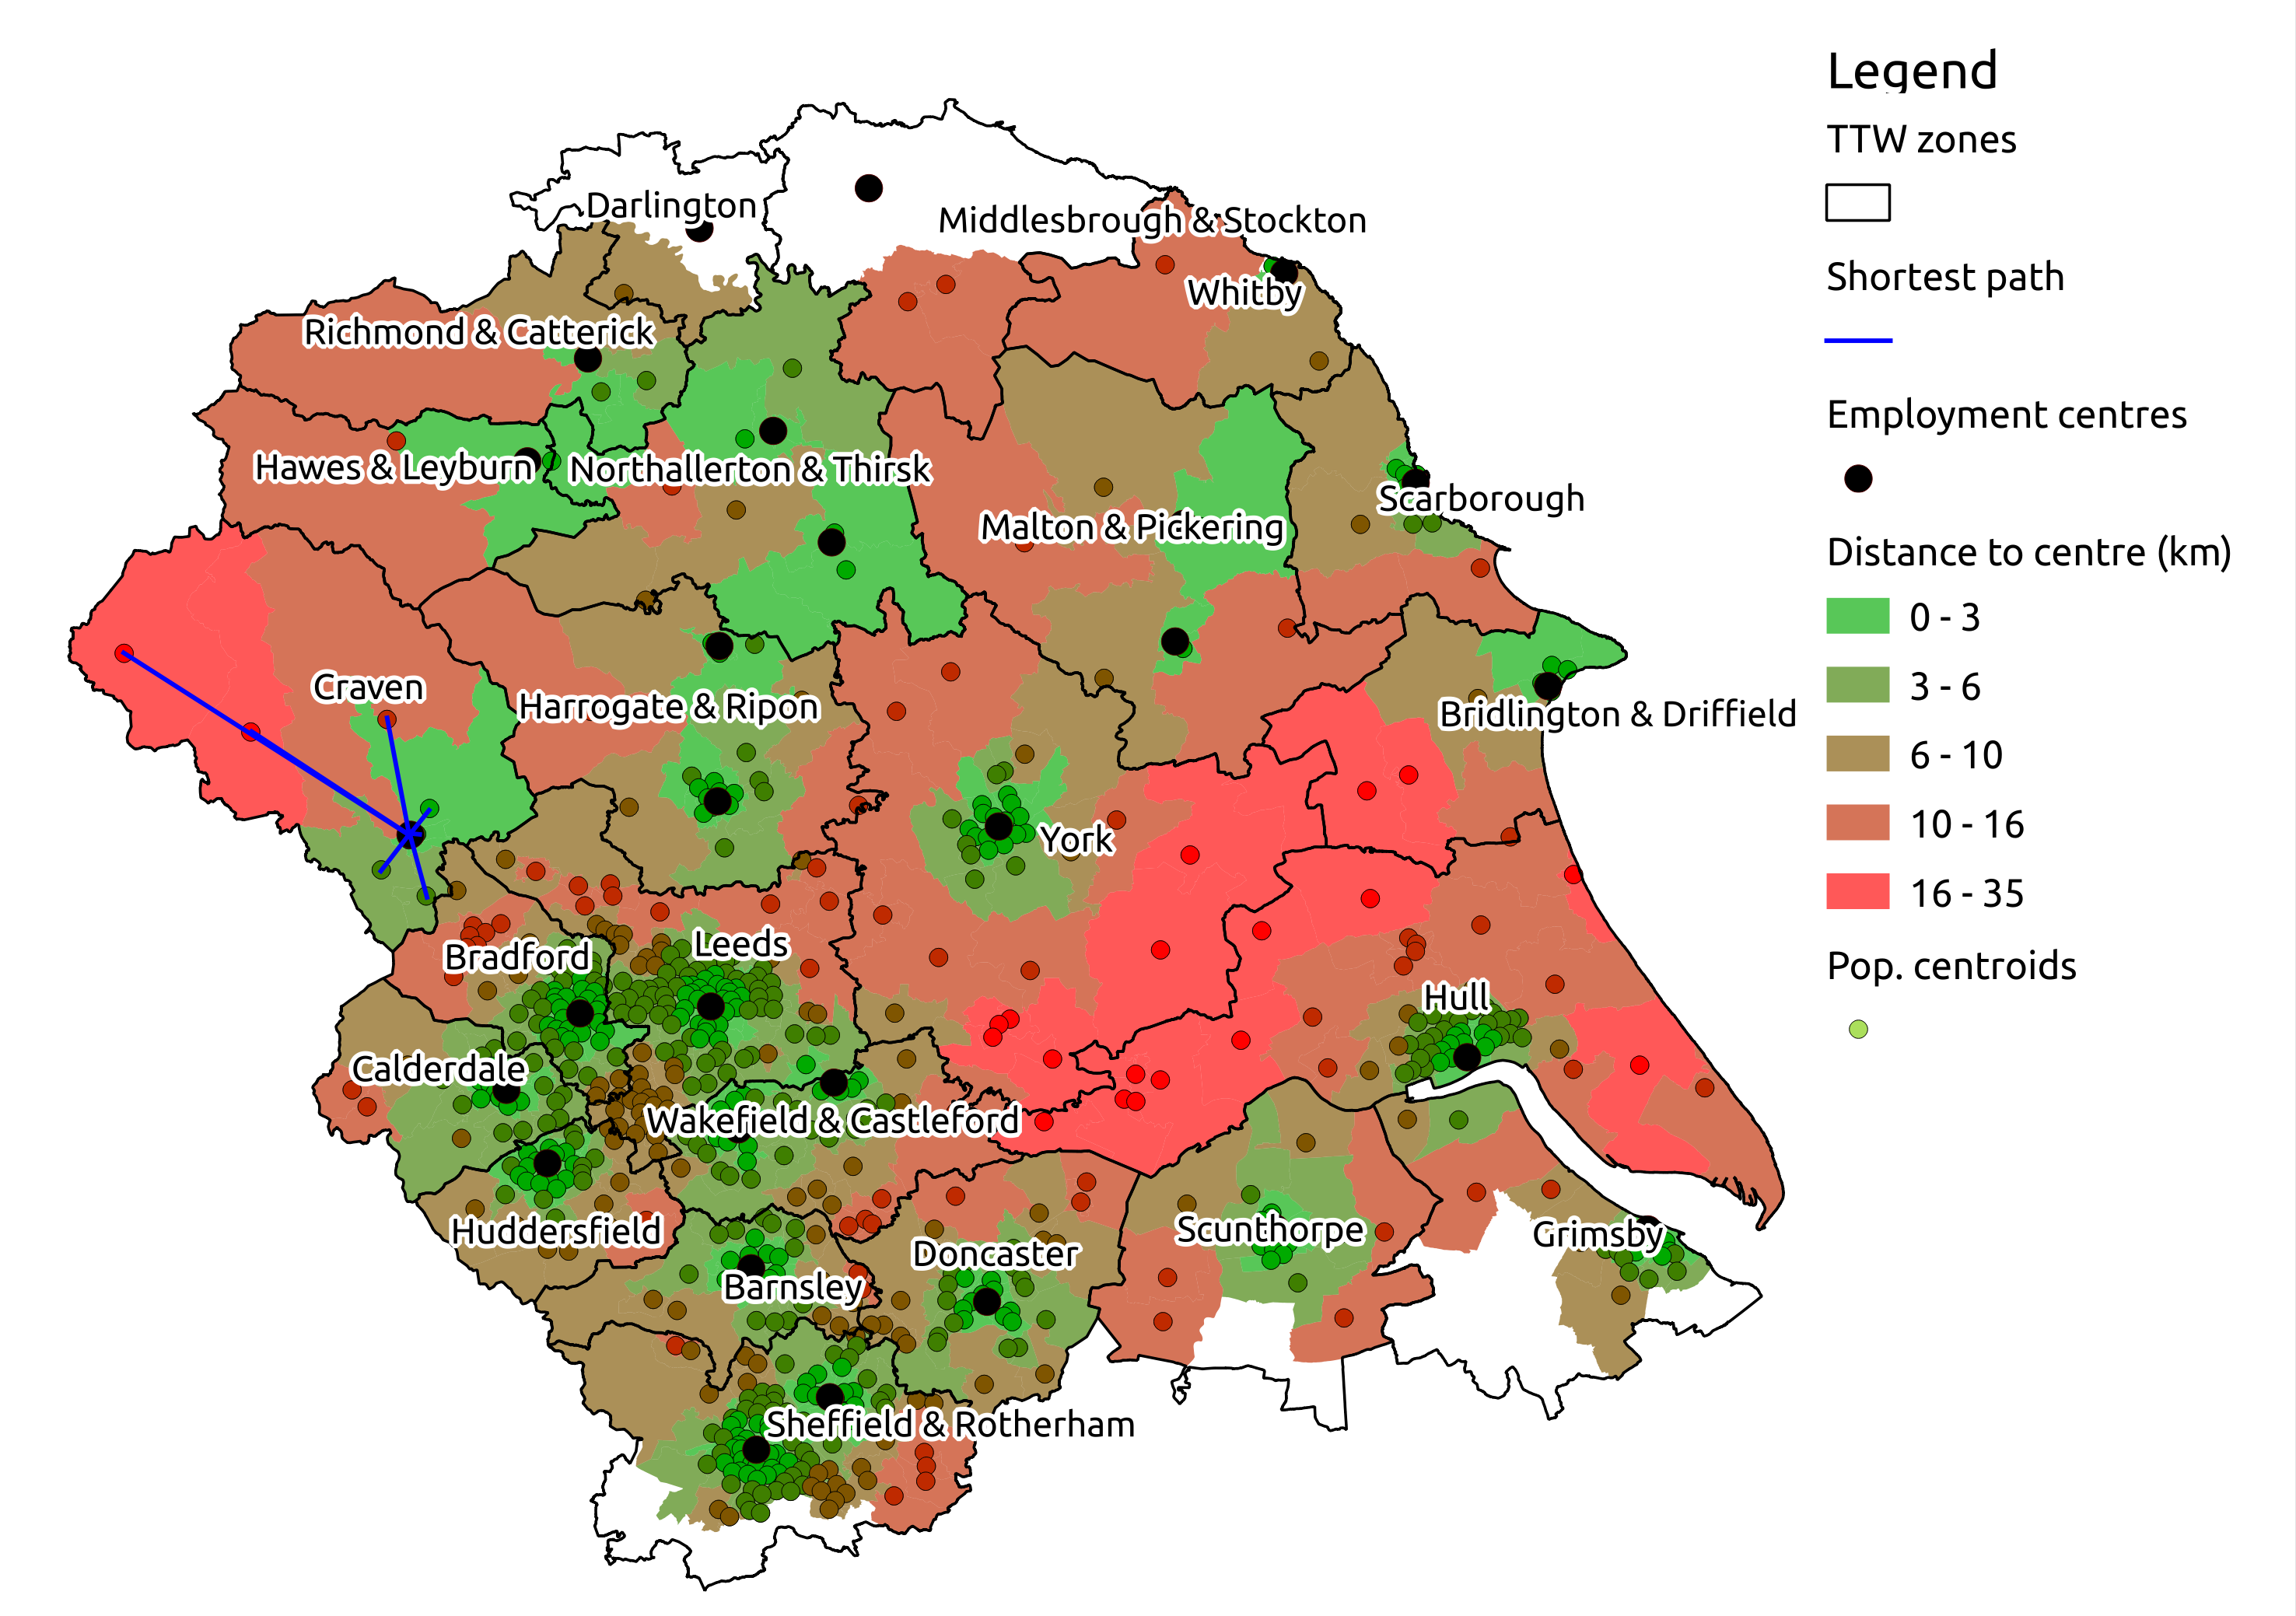
\includegraphics[width=13cm]{Distance-msoa3.png}
 % Graph-line.pdf: 516x363 pixel, 72dpi, 18.20x12.81 cm, bb=0 0 516 363
 \caption[Distance to employment centre from zone centroids]{Distance to
employment centre, calculated as the shortest distance
between zone population centroids and TTW zone employment centres (see
blue lines, which illustrate this calculation for zones in Craven TTW zone).
 Compare with Fig.~\ref{fig:ve}.}
 \label{fig:mapttw}
\end{figure}

So far only geographically aggregated results have been presented.
A key advantage of spatial microsimulation, however, is that individual level
characteristics can be modelled.

\subsection{Local and individual level results}
\label{s:indresults}
The spatial variability described in the previous section
provides insight into the types of places
where commuters are expected to be most vulnerable to oil shocks.
However, high oil prices affect people, not places and a wide range of
commuter habits are present in every area. Geographically
aggregated data therefore only tell part of the story and, if
interpreted incorrectly, can mask intra-zone variability.
In a worst-case scenario this could lead decision makers to
overlook vulnerable groups. Indeed this situation has been described
in Albuquerque, where a new bus network failed to
aid those most in need \citep{Tribby2012}.

Hypothetical commuters illustrate the point. We would expect a
high-income manager, for example, to have a low commuter fuel poverty
($V_{cfp}$)
score due to high income. Their individual level energy vulnerability ($V_{ei}$)
score may be higher, however,
especially if they live in an energy efficient home but drive a large car
many miles to work and back every day, as is common for high earners
\citep{Green-1999-ld-commute}. If they live in a car-dominated area far from
employment centres in a rural `commuter belt', the area in which they live
may well have a high aggregate energy vulnerability $V_e$ score. These
are clearly not the characteristics of a deprived area.
By contrast, an unskilled worker living in a deprived urban area (with a poorly
insulated house) who travels a few kilometres to work may have have a low
$V_{ei}$ but high a $V_{cfp}$ score if they spend
a portion of their low income on expensive bus tickets.

These suppositions may seem obvious but the relative numbers and spatial
distribution of different groups are not. Spatial microsimulation, by estimating
the characteristics of individuals, provides a means of gaining insight into
the likely impacts of oil vulnerability on people beyond aggregated statistics
associated with the areas in which they live. An example of three areas from the
city of York (selected because it is the most unambiguous employment centre
surrounded by countryside in the region) serves to illustrate the point: one is
right in the city centre,
the second is a low income suburb, and the third is on the rural outskirts of
York
(Fig.~\ref{york}).

\begin{figure}[h]
 \centering
   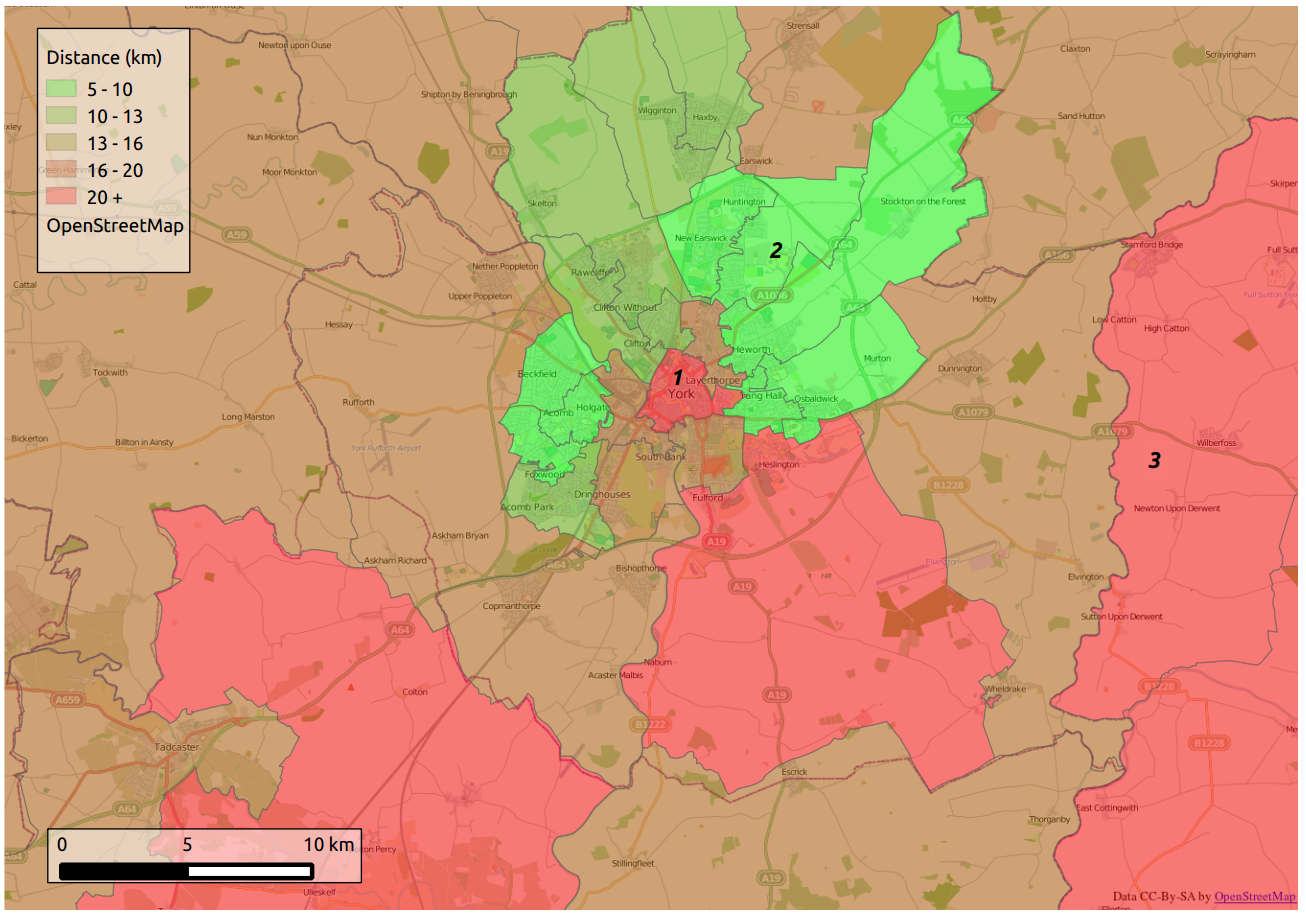
\includegraphics[width=13cm]{york6}
 % Graph-line.pdf: 516x363 pixel, 72dpi, 18.20x12.81 cm, bb=0 0 516 363
 \caption[MSOA zones in York, coloured according to distance travelled to
work]{MSOA zones in York, coloured according to distance travelled to work.
The zones 1, 2 and 3 are referred to below.}
 \label{york}
\end{figure}

Table \ref{t:ind} illustrates summary vulnerability statistics for each of
the three areas numbered in Fig.~\ref{york}, and the average weekly income
for household in each zone.\footnote{The
income estimates are from the Office of National Statistics
Neighbourhood Statistics service. The estimates presented in
Table \ref{t:ind} are the central estimates for equivalised
income from the table ``Income: Model-Based Estimates at MSOA Level, 2007/08''.}
It is interesting to note that the wealthiest zone, in the centre,
is also the most oil vulnerable according to $V_{ei}$ and the second most
vulnerable in terms of $V_e$ and $V_{cfp}$. This finding can be explained
by the high average distance travelled to work by commuters living in the
city centre: wealthy people tend to commute further, leading to higher
energy and monetary expenditure on travel to work. Commuters in the rural
zone (three) commute, on average, the same distance yet they are deemed to
be less vulnerable when vulnerability is measured as the proportion of
people spending more than 10\% of their energy budget
on commuting. This can be explained by the
higher baseline energy use in rural areas \citep{Druckman2008},
meaning that although commuting energy use is high, it does not
form a large proportion of total energy use for most.
The rural zone is most vulnerable in terms of $V_e$, $V_{cfp}$ and $V_h$,
illustrating the importance of income, overall energy use and distance
from employment centre for these metrics.

\begin{table}[htbp]
\caption[Summary statistics of vulnerability metrics]{Summary statistics of
vulnerability metrics and income
estimates for three areas in York. All results presented as
percentages, unless otherwise stated.}
\begin{center}
\begin{tabular}{|l|l|r|r|r|}
\hline
Variable & Statistic & \multicolumn{1}{l|}{1: Central} &
\multicolumn{1}{l|}{2: Suburb} & \multicolumn{1}{l|}{3: Outskirts} \\ \hline
\multicolumn{ 1}{|l|}{Income (\pounds/wk)} & Mean & 440 & 400 & 390 \\ \hline
\multicolumn{ 1}{|l|}{Distance (km)} & Mean & 16.5 & 8.3 & 16.5 \\ \hline
\multicolumn{ 1}{|l|}{$V_{cfp}$} & Mean & 2.0 & 1.1 & 2.1 \\
\multicolumn{ 1}{|l|}{} & SD & 3.5 & 2.8 & 4.9 \\
\multicolumn{ 1}{|l|}{} & $\geq$ 10\% & 3.3 & 1.7 & 5.9 \\ \hline
\multicolumn{ 1}{|l|}{$V_e$} & Mean & 14.9 & 9.1 & 8.4 \\
\multicolumn{ 1}{|l|}{} & SD & 13.9 & 11.5 & 12.3 \\
\multicolumn{ 1}{|l|}{} & $\geq$ 10\% & 55.7 & 32.0 & 28.6 \\ \hline
$V_{ei}$ & - & 17.0 & 10.0 & 18.0 \\ \hline
$V_h$ & - & 3.0 & 9.0 & 33.0 \\ \hline
\end{tabular}\end{center}
\label{t:ind}
\end{table}

Because $V_e$ and $V_{cfp}$ are also calculated at the individual level,
it is possible to estimate the characteristics of vulnerable individuals
at the local level. These results (presented in Table \ref{t:ind2})
illustrate that different types of people are defined as `oil vulnerable'
in different areas. The average income of people living in commuter fuel
poverty (for whom $V_{cfp} \geq 0.1$), for example is much higher in the
city centre than in the outskirts. Table \ref{t:ind2} illustrates that
the characteristics of individuals defined as `oil vulnerable' can also
vary greatly within areas depending on how oil vulnerability is defined.
People living in commuter fuel poverty, for example, tend to be older
than those for whom $V_{cfp} \geq 0.1$. We could hypothesise
whether this is due to a greater reliance
on motorised modes amongst generally less active older citizens or
perhaps also due to lower energy use amongst young people.
Estimates of the average number of children
under the care of commuters were also generated by the model.
These have no bearing on the vulnerability scores, but
illustrate how additional socio-demographic variables could be included to
provide additional information to the simple univariate oil vulnerability
metrics. The distance and mode of school travel, for example, could have a
major impact on the viability of working closer to home in cases where
travel to work is combined with the school run \citep{Hensher2000-chaining}.
%%%!!! ref !!!
Based on the results
from our metrics, it would seem that commuters living in
commuter fuel poverty living in zone 2 and 3 are particularly vulnerable,
with high levels of car dependence yet low incomes.


\begin{table}[htbp]
\caption[Individual level characteristics
of `oil vulnerable' commuters]{Individual level characteristics
of `oil vulnerable' commuters in living in the three zones of
York depicted in Fig.~\ref{york}, estimated by the spatial microsimulation
model.}
\begin{center}
\begin{tabular}{|c|l|r|r|r|}
\hline
Subset & Statistic & \multicolumn{1}{l|}{1: Central} & \multicolumn{1}{l|}{2:
Suburb} & \multicolumn{1}{l|}{3: Outskirts} \\ \hline
\multicolumn{ 1}{|c|}{$V{cfp}$} & N & 241 & 51 & 151 \\ \cline{ 2- 5}
\multicolumn{ 1}{|c|}{$\geq 10\%$} & Average age & 39 & 41 & 44 \\ \cline{ 2- 5}
\multicolumn{ 1}{|c|}{} & Average income & 19100 & 15800 & 14300 \\ \cline{ 2-
5}
\multicolumn{ 1}{|c|}{} & Income SD & 9400 & 10100 & 8400 \\ \cline{ 2- 5}
\multicolumn{ 1}{|c|}{} & N. children & 0.51 & 0.88 & 0.67 \\ \cline{ 2- 5}
\multicolumn{ 1}{|c|}{} & \% drive to work & 45 & 53 & 56 \\ \hline
\multicolumn{ 1}{|c|}{$V{e}$} & N & 1168 & 990 & 2466 \\ \cline{ 2- 5}
\multicolumn{ 1}{|c|}{$\geq 10\%$} & Average age & 35 & 31 & 41 \\ \cline{ 2- 5}
\multicolumn{ 1}{|c|}{} & Average income & 18000 & 16600 & 19200 \\ \cline{ 2-
5}
\multicolumn{ 1}{|c|}{} & Income SD & 11900 & 8000 & 10300 \\ \cline{ 2- 5}
\multicolumn{ 1}{|c|}{} & N. children & 0.67 & 0.64 & 0.67 \\ \cline{ 2- 5}
\multicolumn{ 1}{|c|}{} & \% drive to work & 43 & 40 & 61 \\ \hline
\multicolumn{ 1}{|c|}{All } & N & 4085 & 3091 & 4424 \\ \cline{ 2- 5}
\multicolumn{ 1}{|c|}{commuters} & Average age & 36 & 41 & 42 \\ \cline{ 2- 5}
\multicolumn{ 1}{|c|}{} & Average income & 19500 & 17900 & 19686 \\ \cline{ 2-
5}
\multicolumn{ 1}{|c|}{} & Income SD & 12600 & 10800 & 12000 \\ \cline{ 2- 5}
\multicolumn{ 1}{|c|}{} & N. children & 0.56 & 0.7 & 0.67 \\ \cline{ 2- 5}
\multicolumn{ 1}{|c|}{} & \% drive to work & 25 & 49 & 61 \\ \hline
\end{tabular}\end{center}
\label{t:ind2}
\end{table}

By providing estimates for a range of individual level variables, spatial
microsimulation can highlight the various types oil vulnerability.
Returning to the two hypothetical commuters mentioned at the beginning of
the section, one could further predict their relation to policy interventions.
Policies encouraging telecommuting
may be more effective if targeted towards the manager (with the potential
co-benefit of freeing up oil for shorter commutes or public transport). The
unskilled worker, by contrast, may be better served by pro-cycling policies
or subsidised buses to
increase the viability of cheaper and more active forms of
travel. (Public transport is generally more active than driving, as people
tend to walk to and from bus stops \citep{Besser2005-active}.)
Based on a dynamic spatial microsimulation models, the local impacts of these
policies could be projected \citep{Ballas2005-ireland}. As with
aggregate measures, commuter oil vulnerability at the individual level clearly
has
multiple meanings and interpretations.
The model results support this view and could, if combined with additional
vulnerability metrics (e.g.~those used in the IMD),
be used as a multifaceted concept oil vulnerability overall.

\section{Discussion: policy relevance and limitations}
\label{fc8discus}
In this chapter the potential of the spatial microsimulation approach
for the analysis of commuter patterns 
for informing policy has been tested. Three `what if' scenarios of change
leading to lower commuting energy costs have been developed and two of
these have been quantified, yielding interesting and policy-relevant results.
The first aim of this thesis, set out in \cref{s:aims}, was to not
only investigate the variability of commuter energy costs, but also its
policy implications. The previous two results chapters also have policy-relevant
findings, but it is only here that scenarios of change in commuting patterns
have been evaluated in energy terms. As set out in \cref{Chapter1}, the
motivation behind this research was to some degree political: the perceived
need for policies to rapidly reduce the rate at which fossil fuels are burned,
to avoid the worst impacts of climate change and fuel depletion.
It is easy to say that such policies are needed in the transport sector
\citep{Chapman2007}, but quite another to select precisely which policies
are likely to be most effective at achieving this
aim.\footnote{Indeed, \citet{Berners-Lee2013}
show that many well-intentioned efforts to reduce emissions have
a tendency to simply displace emissions to a different time or place
(they liken trying to reduce emissions to `squeezing a balloon' --- it
always bulges out somewhere else). To provide one example in the context
of commuting, the shift to electric cars certainly reduces direct emissions
at the point of use, but may increase emissions at the power plants that
charge the batteries, and in the mines, factories and freight transport
networks than are needed to produce electric cars. 
}
The second aim  was to ``Formulate and analyse scenarios of change''.
This has been achieved for case studies in South Yorkshire, based on the
potential of commuters to shift mode to bicycles and reduce the frequency
of their trips to work through telecommuting. Other plausible scenarios of
change could have been developed, such as increases in car sharing, and
shifts to other forms of transport.
Both of these options have great potential to reduce energy costs of commuting
in the short-term, but were not formalised as quantitative scenarios due to
data and time constraints in the first case and the fact that widespread
investment in public transport, high speed railways notwithstanding,
currently seem a remote possibility in the 
latter.\footnote{The
potential of car sharing depends
not only on the number of people driving similar distances to work, but also the
direction of travel. This data is not included in the spatial microsimulation model
presented thus far, although it is available at Output Area and Ward levels,
as described in \cref{s:workdes}. Car sharing, it is hypothesised, has great
potential to reduce commuting energy costs, as it allows long distance trips
to be tackled, forming an interesting future direction for this research.
The replacement of car journeys with public transport also has great potential
as buses, coach, trams and trains are far more efficient than cars. However,
during this time of fiscal constraint, it seems unlikely that the large-scale
roll-out of new public transport services that this scenario would require
will happen any time within the next decade or so. In fact, some bus services
are in jeopardy of being cut altogether due to financial pressure \citep{Owen2012}.
}
The spatial microsimulation method could be used for evaluating many other
scenarios of policy intervention, and can estimate change in many other variables
beyond energy use. The likely distributional impacts of proposed policy interventions
is an area where the method has greatest potential for policy influence.
Although there are many other unexplored scenarios that could usefully be
evaluated using spatial microsimulation, a strong argument can be made that
the results generated in this chapter are interesting and relevant in themselves.

\subsection{Policy relevance of findings}
A substantial shift to bicycles in England (with bike
trips reaching 10\% of all trips to work) was modelled by the `go Dutch' scenario.
This would affect around 13\% of the population (and 14\% of car drivers)
but only reduce commuter energy use by 3\%, an unexpectedly low figure for
such a dramatic shift.
Perhaps this surprise comes primarily as a result of preconceptions of the
bicycles as being a `green' mode of transport: it is
often assumed that promoting this mode of transport will lead to
large and rapid reductions in energy use and associate
emissions.\footnote{Studies
that
have quantified the likely savings tend to have similarly pessimistic
findings, however: that potential energy and emissions savings from bicycling
uptake alone are small in the grand scheme of things. \citet{Lovelace2011-assessing}
found maximum savings of only 90 MJ/person/yr (less than 0.1 kWh/p/day, well
around 0.1\% of current per capita energy use in the UK) by 2020 even under
the most optimistic cycling scenario in one city. \citet{Lindsay2011}
found that ``Shifting 5\% of vehicle kilometres to cycling would reduce
vehicle travel by approximately 223 million kilometres each year, save
about 22 million litres of fuel and reduce transport-related greenhouse emissions
by 0.4\%'', a strikingly similar finding given that transport
causes around 1/4 of emissions. 
}
The
results suggest than more than uptake of cycling
is needed for substantial reductions in energy use in the current system.
% While I remember: correlate this with energy use per region!!!
% Also the kinds of people affected !!!
In addition, it was found that the greatest savings would accrue to individuals
(who drive short distances to work) and areas (located near to employment
centres) that have relatively low energy costs for commuting \emph{already}.

In the `go Finnish' telecommuting scenario, by contrast, altering the
behaviour of a small proportion of the population was found to have a
disproportionately large effect on total energy use in the case study region.
% Same here: it's crying out for tables
Because a switch to telecommuting is more likely amongst long-distance commuters,
and long-distance commuting is associated with higher incomes, it
can be inferred that policies that promote telecommuting would be
`energetically progressive', affecting those who already use most energy the most.
Pro-cycling measures, on the other hand, could be seen as `energetically
regressive' based on the results presented in this chapter: only people
who already live relatively close to home are, in general, able to switch to
cycling. None of this is to say that cycling promotion is `bad' per se,
simply that its energy and environmental benefits may not be as great as
expected, and lower than policies which target the most energy intensive
commuters. Differences between the individuals affected by the `go Dutch'
and `go Finnish' scenarios are illustrated in \cref{tdifscens}. This table
shows that the distribution of climate/energy policies vary widely in
the transport sector: those affected by the telecommuting policy have
a substantially higher average income than those affected by the pro-bike
scenario. One could argue that they would be better able to deal with the
resulting effects. Most strikingly, the results show that those affected
by the cycling scenario already use quite little energy for their daily commute,
whereas those who take up telecommuting use on average more than 3 times more
energy per trip to work than the county-wide average. In energy terms,
the `go Dutch' scenario is regressive, whereas the `go Finnish' scenario is
progressive. That's not to say that the latter is `better' --- energy and
emissions will be only one of several considerations taken into account.
The analysis suggests that the two policies would complement each other well:
The areas of greatest energy savings from a shift to bicycles tend to be close
to city centres where many people commute a short distance by car.
Telecommuting, by contrast will have most impact in commuter belts far from
urban centres.
% Add in correlation in energy savings between the two here

\begin{table}[htbp]
\caption[Differences between commuters affected by the `Dutch' and `Finnish' scenarios]
{Differences between commuters affected by the `Dutch' and `Finnish' scenarios, expressed
as averages over all commuters in South Yorkshire}
\centering{\begin{tabular}{lrrr}
\toprule
Variable & \multicolumn{1}{l}{All commuters} & \multicolumn{1}{l}{`Go Dutch'} & \multicolumn{1}{l}{`Go Finnish'} \\
\midrule
\% affected & 100 & 8 & 2.8 \\
Etrp (MJ/trip) & 39 & 22 & 134 \\
Income (\pounds) & 18090 & 17910 & 24357 \\
Age & 39 & 40 & 41 \\
Distance (km) & 11 & 5 & 33.5 \\
Energy saving (\%) & 0 & 2.8 & 9.2  \\
\bottomrule
\end{tabular}}
\label{tdifscens}
\end{table}

The final scenario was by far the most ambitious. `Eco-localisation', it was
decided, would occur long in the future. People would have different
attributes, the distribution of jobs would be different and the
entire structure and function of urban systems may have changed
due to previously unforeseen processes and events (some driven by technology,
others by unexpected `black swan' incidents \citep{Korowicz2011}). Based
on these features of this final scenario, it is difficult to model. It was
decided that the spatial microsimulation approach set-out in \cref{Chapter4}
would not be appropriate to estimate the energy savings of this scenario, as
it would simply be a function of the author's (subjective) assumptions about
what a more localised economy would look like in terms of commuting.
As Vaclav Smil has pointed out on several occasions (e.g.~\citeyear{Smil1993, Smil2010}),
there are limits to quantification and modelling, and these are especially
applicable in long-term forecasts on the basis of which decisions must be made.
It is important to consider these limitations lest the results be misinterpreted,
leading to ineffective policies. Many of the limitations of the approach
expounded in this thesis are well-exemplified by the eco-localisation
scenario, which would push any modelling approach to its limits.

\subsection{Limitations of the approach} \label{s:uncertainties}
Firstly, it is vital to remember that we are dealing with \emph{virtual}
individuals, whose characteristics have been simulated based on a set of
constraint variables. Even the total population represented by these individuals
in each area is not completely objective: the total number varies in our
dataset from one constraint to the next so one must be selected (in this
case mode of travel) and the others set equal to this. Beyond this minor issue
the constraint variables (and total counts within each constraint category)
can be relied upon as accurate if the process of spatial microsimulation
works properly and the IPF converges properly to a single result (see
\cref{meval}): census data are highly reliable, and the correct number
of individuals with certain characteristics will be selected.

A critical distinction must be made when using data generated by
spatial microsimulation: between the aforementioned constraint variables and
target variables that are unconstrained. Income is a good example of a target
variable because it is clearly linked to age, sex, distance and mode of travel to work and
especially to social class, but is not totally determined by these constraints.
The high (r $\sim$0.8) correlation between official average income estimates and those generated
by the spatial microsimulation presented in \cref{fig:income-test} provide confidence
that the model is working correctly but also raise the question: what accounts for the
other 20\% of variability in average income between wards?
The answer is that the model, based on the current constraints, cannot tell us.
Even if more constraints such as car ownership and tenure were added, still not all of
income variability would be accounted for at the aggregate level, let alone the local
level. Reality is complex, and it must be acknowledged that models cannot (and probably
should not) attempt to encapsulate the totality of the interacting, sometimes unquantifiable
factors that are at work. In this context, the energy use variable that has been
calculated for individuals and regions is `semi-constrained'. By this is meant
that the main mode and (crudely binned) euclidean distance band for
individuals' \emph{usual} (not constant) trip to work is known. These two
factors are the
most important controls on energy use \cref{Chapter5} and are constrained by
census data, so the estimates are likely to reflect the reality of commuter
energy use to a large extent. 

The second critical limitation of the approach with respect to future scenarios
is that it is static. No dynamics are included in the model, so the only way future
change can be represented is by updating the constraint variables and holding
everything else constant, or by selecting individuals based on certain attributes
who are deemed to be most likely to switch behaviour, as done here. This approach
has the benefit of simplicity, clarity and transparency, yet lacks the sophistication
of agent-based models.
% Still, modelling a system that is `on the edge of chaos'
% transition to a completely new state is always going to rely on a number of
% un-testable assumptions.

Beyond these issues of interpretation and the need to develop carefully constructed
assumptions for the model to be of use to policy-makers, spatial
microsimulation, as implemented in this thesis, lacks the sophistication and
detail of the recent breed of agent-based transport models. MATSim, for example,
can include individual level characteristics, model trip demand \emph{and}
allocate
this demand to the transport network in near-continuous time \citep{Balmer2009}.
On the other hand, such detail and sophistication comes at a cost: MATSim
may be harder to configure and interpret than the comparatively simple approach
taken here. Also, coming from the transport perspective, transport models
tend to be inherently less interested in distributional impacts than impacts
on road traffic, although distributional impacts could still be built in
provided appropriate input data (with socio-economic variables) is used.
This raises the possibility of using the output of the spatial microsimulation
approach advocated in this thesis as an input into more advanced model,
something that is further considered in the conclusion.

The final limitation of the modelling approach that has already been alluded to,
and that to some extent afflicts all models that are built on static
assumptions about the world, is the potential of unexpected events to render
them ineffective. An `oil shock' is one example of this, that has already been
tackled, in \cref{svul}. One near-certainty about the future, however, is
that climate change will continue to produce weather that is extreme by
historical standards \citep{Koetse2009}.
% It is to this topic, and the potential for impacts on
% transport, towards which attention is now directed. In this context an
% indirect feedback loop can be observed, whereby transport emissions affect
% the climate, which in turn affects transport systems.

% \subsection{Climate change impacts on commuter infrastructure}
% \label{s:uncertainties}
% Not only does energy intensive commuting \emph{affect} climate change, it
% is also \emph{affected} by changes in climate variables, in a number of ways.
% This side of the two way relationship may well be the more important at the
% national level, because
% UK emissions from commuting make up less than 0.1\% of the global total. Yet
% the potential impacts of climate change on commuter patterns is great.
% Consideration of these possibilities is useful not only to place commuter
% energy use in its broader context of 21$^{st}$ century change, but also to
% illustrate the uncertainties surrounding the future of motorised transport in
% the UK. (\Cref{fig:ccsum} and \cref{fig:ccpdf}) illustrate
% the large uncertainties associated with changes in UK average temperatures (the
% best understood climate variable), and
% the dependence of forward projections on scenarios of the future.
% \begin{figure}[htbp]
%   \centering{
%     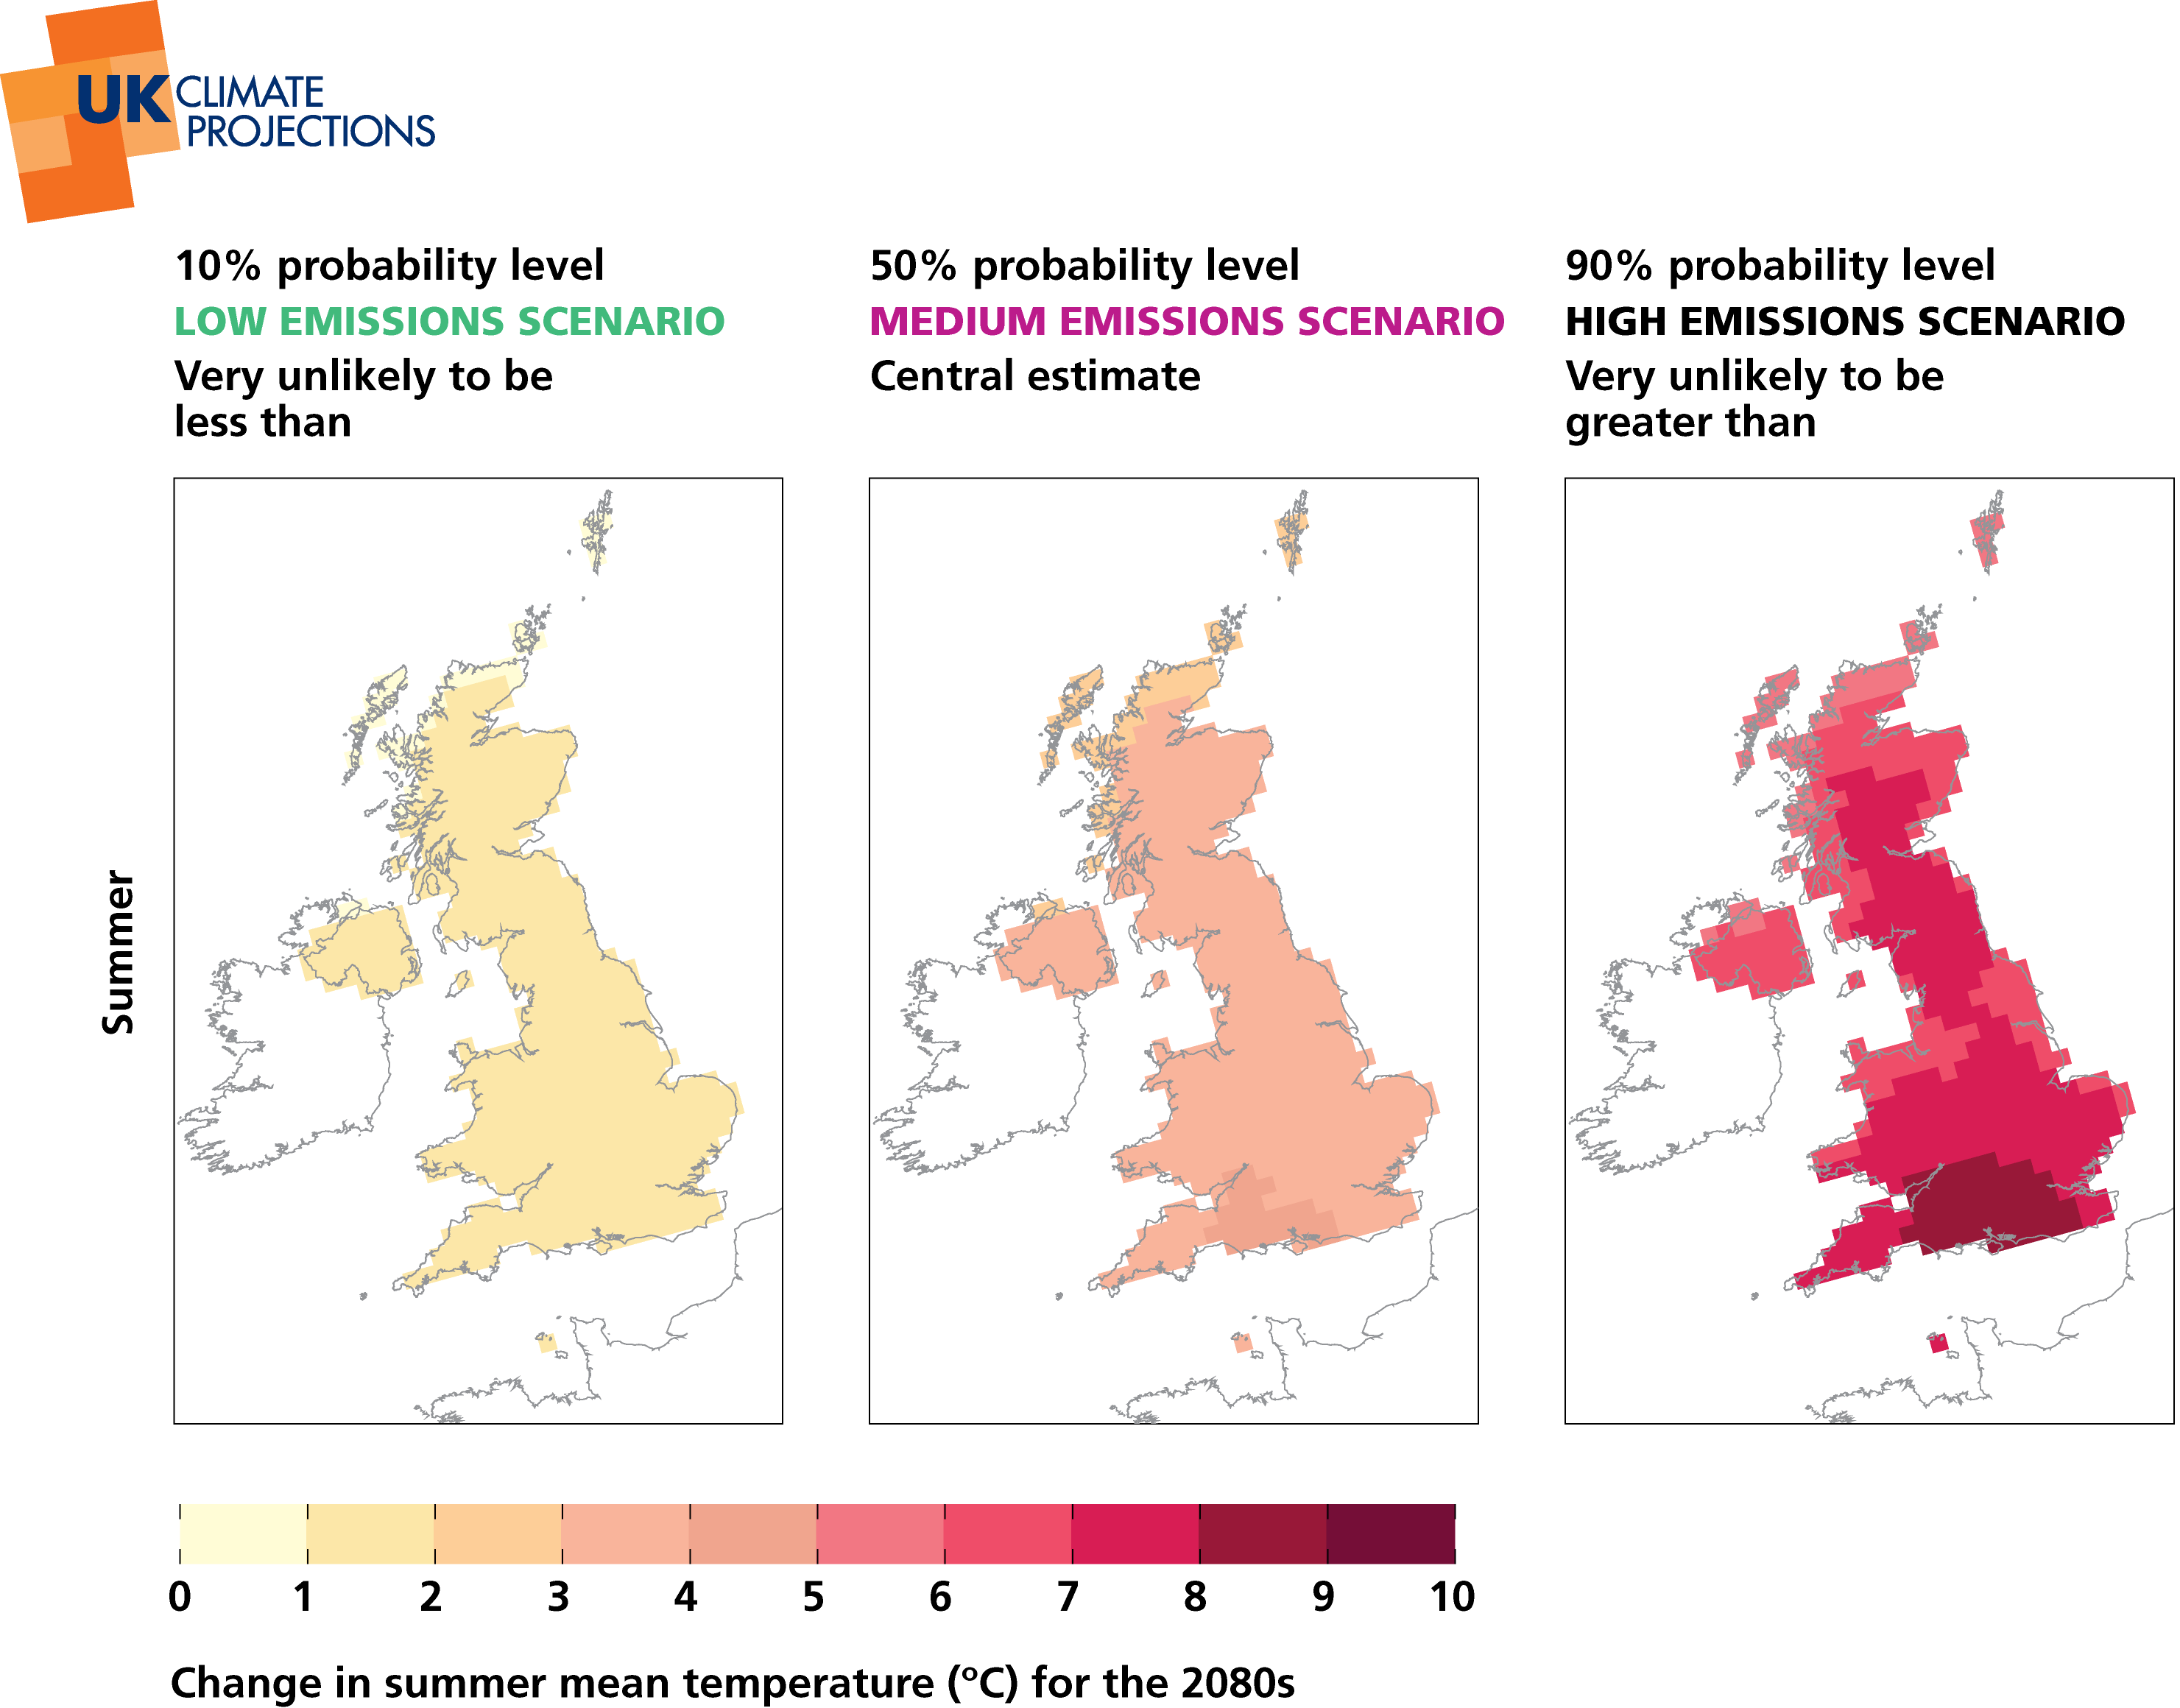
\includegraphics[width = 14 cm]{./Figures/cc-sum.png}}
%   \caption[Climate change in the UK]{Range of projected summertime temperature
% anomalies in the UK, depending on different emissions scenarios
% \citep{Murphy2009}}
%   \label{fig:ccsum}
% \end{figure}
% 
% \begin{figure}[htbp]
%   \centerline{
%     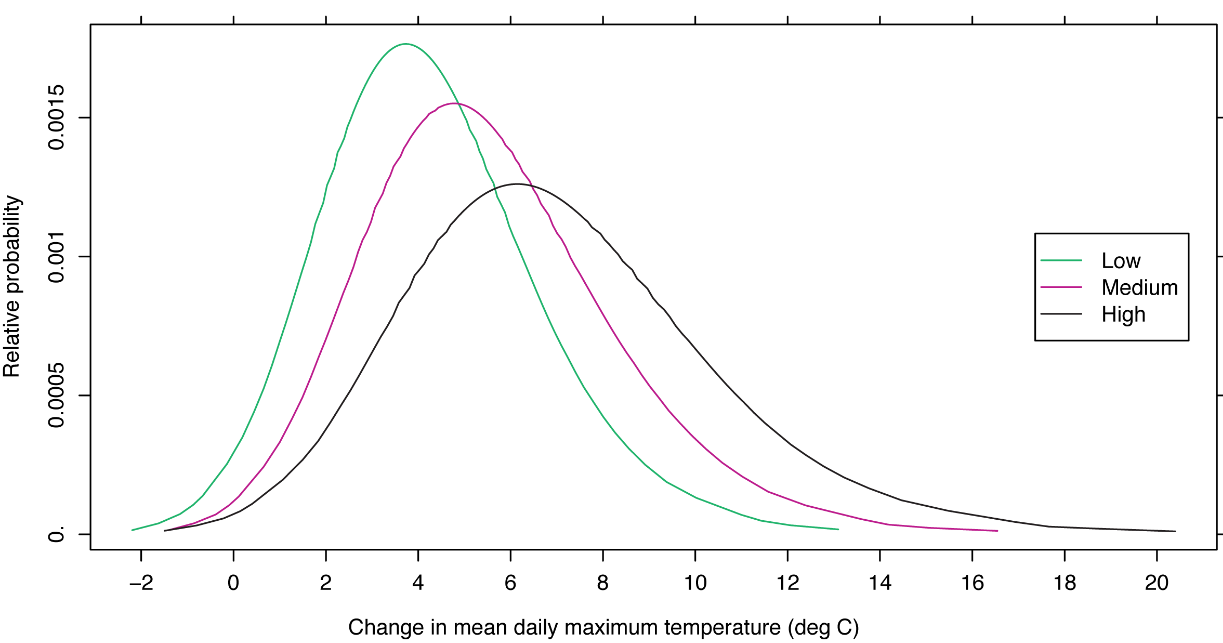
\includegraphics[width = 14 cm]{./Figures/cc-pdf.png}}
%   \caption[UK climate change scenarios]{Probability distributions of temperature
% increases following 3 different emissions scenarios in the UK. Low, medium and
% high scenarios refer to the IPCC emissions
% scenarios B1, A1B, and A1FI, respectively (see \citealp{Nakicenovic2000})}
%   \label{fig:ccpdf}
% \end{figure}
% 
% The range of temperatures projected in \cref{fig:ccsum} represent the
% extreme lower, middle, and extreme upper ends of average UK temperature change,
% in comparison with the 20$^{th}$ Century average \citep{Murphy2009}. Such a
% wide range of possibilities is due both to model uncertainty, and uncertainty
% about the future rate of worldwide greenhouse gas emissions.
% 
% The scope for impacts on transport systems and infrastructures is great,
% ranging from small changes at the local level to disruption of oil supplies
% caused by extreme weather. A survey of the
% literature on the subject suggests the following issues, of relevance to
% commuting, are of particular concern \citep{Koetse2009}:
% \begin{itemize}
%  \item Damage to road and railway infrastructure due to sea level rise and an
% increased incidence of storm surges associated with climate change. In the UK,
% this would be likely to affect large areas of coastal lowland in the Thames and
% Humber estuaries \citep{Shennan1993}.
% \item Indirect impacts of increased flooding. These would likely include
% ``delays, detours and trip cancellation'' \citep{Koetse2009}.
% \item The impacts of sea level rise and extreme weather on freight patterns
% could have knock-on impacts for commuters. Discussion of these impacts is
% purely speculative \citep{Koetse2009}, but could include the disruptions in the
% supply of oil and economic turmoil \citep{Curtis2009}.
% \item Warmer drier summers and warmer winters in the UK predicted by
% \citet{Murphy2009} could encourage the uptake of walking and cycling.
% \end{itemize}

In summary of this chapter, it has been shown that
scenarios about the future can
be modelled by a spatial microsimulation model of commuters, with important
policy implications. It is important to acknowledge the limitations of this
approach, however, which include its use of simulated individuals who
may differ from real people, and its treatment of an uncertain future.
Overall great progress has been made towards meeting the aims of the thesis.
% These aims are returned to in the
% subsequent and final chapter.
% !!! move the stuff about aims into the conclusion, right???

% \begin{figure}[htbp]
%   \centerline{
%     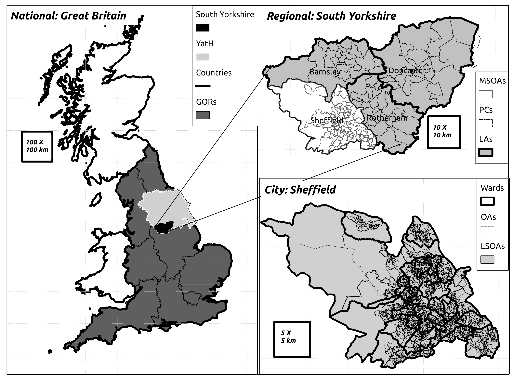
\includegraphics[width = 14 cm]{scales-map-low}}
%     \rule{35em}{0.5pt}
%   \caption{Case study region}
%   \label{fig:sarea}
% \end{figure}

% 
% % Chapter 8 - evaluate!
% Spatial microsimulation cannot replace the `gold standard' of real,
% small area microdata \citep[p.~4]{Martin2002}. However, the method's practical
% usefulness (see \citealp{Tomintz2008}) and testability \citep{Edwards2009} are
% beyond doubt. Assuming that the microdataset is representative of the
% individuals living in the zones under investigation,\footnote{The suitability
% of this assumption is further discussed in \cref{Chapter8
